%% Document class (Koma Script) -----------------------------------------
\documentclass[%
   %draft,						% under-/overfull boxes are marked with black square, no pictures
   final,							% final document
%%%% === Font Size ===
   12pt,
%%%% === Language ===
   english,	german				% delegated to other packages
%%%% === Page Size ===
   % letterpaper,
   % legalpaper,
   % executivepaper,
   a4paper,
   % a5paper,
   % landscap,
%%%% === Options for type area ===
   BCOR1cm,						% Binding correction offset
   DIV11,							% Page Size (see Koma script documentation!)
   DIV=calc,					% automatic line length calculation
   1.1headlines,			% Line count for head
   %headinclude,			% include head into calculations
   headinclude=false,	% exclude head from calculations
   footinclude=false,	% exclude foot from calculations
   mpinclude=false,		% exclude margin from calculations
   pagesize,					% write page size to document file
											% Important for correct size conversions
%%%% === Layout ===
   oneside,						% one-side layout
   %twoside,					% side margins for two-side layout
   onecolumn,					% single column layout
   %twocolumn,				% double column layout
   %openany,         	% chapters may start on any page
   openright,					% chapters may only start on a right side (unimportant for oneside layouts)
	 headings=big,			% choices: small, normal, big
   										% print headings in appendix like others
   										% onelineappendix, noappendixprefix, appendixwithoutprefix, appendixwithoutprefixline
   										% print chapter headings like others
   										% onelinechapter, nochapterprefix, chapterwithoutprefix, chapterwithoutprefixline
   										% print headings in appendix with additional prefix line
   										% twolineappendix, appendixprefix, appendixwithprefix, appendixwithprefixline
   										% print headings in chapter with additional prefix line
   	chapterprefix,					% twolinechapter, chapterprefix, chapterwithprefix, chapterwithprefixline
   										% openany: \clearpage not \cleardoublepage after chapters, index, etc.
   										% openleft: \clear-commands may produce page break & start chapter on left page
   										% openright: \clear-commands may produce page break & start chapter on right page
   										%
   captions=oneline,	% seperate handling of one-line captions --> centered
	 %captions=nooneline,% no seperate handling of one-line captions
	 %captions=heading,	% captions of floating environments are formatted as headings, placement dependent on
	 										% \caption{} position!, equal to above & top, implicate captions=tableheading|figureheading
	 %captions=signature,	% captions of floating environments are formatted as headings, placement dependent on
	 										% \caption{} position!, equal to above & top, implicates captions=tablesignature|figuresignature
	 %captions=figureheading,	% figures will have their caption 'on top', equal to figureabove, abovefigure,
	 													% topatfigure, typographically undesirable!
	 %captions=figuresignature	% figures will have a trailing caption, equal to belowfigure, bottomatfigure
	 													% this is what you want! (caption will be formatted as captionbelow)
	 captions=tableheading,		% tables will have their caption 'on top', equal to tableabove, abovetable,
	 													% abovetabular, topattable, this is what you want! (caption will be formatted as captionabove)
	 %captions=tablesignature	% tables will have a trailing caption, equal to belowtable, belowtabular, bottomattable
	 										%
	 										% other caption options: topbeside, bottombeside, centeredbeside, innerbeside, outerbeside,
	 										%	leftbeside, rightbeside
   cleardoublepage=plain,	% empty left side mit page style 'plain'
   %cleardoublepage=empty,	% empty left side mit page style 'empty'
   titlepage,					% title as standalone page ('titlepage' environment)
   %notitlepage,			% title integrate in other page
%%%% --- Paragraph Indentation ---
   %									% Paragraph spacing: single-spaced
   parskip=true,			% options:
   										% full|true|on|yes: paragraphs denoted by 1 line vertical spacing, no indentation
   										% full-						: paragraphs denoted by 1 line vert. spacing, ends undenoted
   										% full+						: paragraphs denoted by 1 line vert. spacing, ends with third of a line spacing
   										% full*						: paragraphs denoted by 1 line vert. spacing, ends with quarter of a line spacing
   										% half						: paragraphs denoted by 1/2 line vert. spacing, ends with third of a line spacing
   										% half-						: paragraphs denoted by 1/2 line vert. spacing, ends undenoted
   										% half+						: paragraphs denoted by 1/2 line vert. spacing, ends with third of a line spacing
   										% half*						: paragraphs denoted by 1/2 line vert. spacing, ends with quarter of a line spacing
   										% false|off|no		: paragraphs denoted by indentation
   										% never						: no spacing between paragraphs
%%%% === Header ===
%
   headsepline=true,	% line below header
   footsepline=false,	% no line above footer
%
%%%% === Lists (TOC, LOF, LOT, BIB) ===
%
   toc=bibliography,	% include bibliography in table of contents unnumbered
   										% alternatives:	bib, bibliographynumbered, bibnumbered
   										% 							nobibliography, nobib	
   toc=index,					% include index in table of contents (idx & similar options as with bib)
   toc=listof,				% include list of figures|tables|algorithms|etc. in TOC
   										% alternatives: listofnumbered, numbererdlistof, nolistof
   toc=indented,			% indented TOC, equal to graduated, indent
   %toc=left,					% table-like TOC, equal to flat
   numbers=autoendperiod,	% automatic headline enumeration w/ & w/o end period
   										% german users: see DUDEN R3|R4
   										% other option noendperiod, endperiod (manual)
   %openbib,					% alternate bibliography style
%
%%%% === Equations ===
%
   %leqno,						% equation numbering on the left side
   fleqn,							% equations are printed flushed left
]{scrreprt}						% all classes: scrartcl, scrreprt, scrbook
\usepackage{scrhack}	% get rid of warning due to packages incompatible with KOMA script
%
%
% General
%
\usepackage[T1]{fontenc}
\usepackage[utf8]{inputenc}
\DeclareUnicodeCharacter{FEFF}{}
\usepackage[ngerman]{babel}
%\usepackage[latin1]{inputenc}
%\usepackage[ansinew]{inputenc}														% umlauts in editor
\usepackage{lmodern}																			% Type1-font for non-english texts
\usepackage[bindingoffset=0cm, top=2.5cm, left=3cm, right=3cm]{geometry} % page margins
%\setcounter{tocdepth}{3}																	% set depth of table of content
%\setcounter{secnumdepth}{5}															% set depth of section numbering
\usepackage{amssymb}																			% provides mathmatical math symbols such as dots, arrows, etc.
\usepackage{amsmath}																			% provides align environment
\usepackage{dsfont}	
\usepackage{ngerman}																		% double stroke font for number set symbols, (N, Z, Q, R, C)
\usepackage[german,intoc]{nomencl}												% create list of abbreviations (add it to TOC)
\usepackage{datetime}
\usepackage{booktabs}
\usepackage{imstitle}

%
% Layout
%

% Remove the dot after the chapter number
\renewcommand*{\chapterformat}{%
  \chapappifchapterprefix{\nobreakspace}\thechapter%
}
\usepackage{microtype} % avoids most of overlong lines by adjusting interword space
\usepackage[automark, headsepline, autooneside]{scrpage2}	% header seperated via line
% Setup header & footer
\renewcommand*{\chapterpagestyle}{plain} % pages starting a new chapter only have a page number
\renewcommand*{\titlepagestyle}{plain} % title page only has page number
\renewcommand*{\indexpagestyle}{plain}	% all lists shall show the page number
\pagestyle{scrheadings}
\clearscrheadfoot																					% reset header & footer fields to NULL
\ohead[\pagemark]{\pagemark} % display page number on the outside
\ihead[]{\headmark}	 % section or subsection on the inside
%\automark[chapter]{chapter} % use section as header text
\usepackage{float} % provides H as placing option, use with caution!
\usepackage{setspace} % easy way to set 1x, 1.5x or 2x line spacing
\usepackage{parskip} % paragraph separation: indentation -> smal line

%
% Graphics
%
\usepackage{wrapfig}
\usepackage[pdftex]{graphicx}															% use bmp|jpg|png|pdf within \LaTeX
% color must appear AFTER graphicx!
\usepackage{color}																				% provides colors such as Black, Blue etc.
%\usepackage[caption=false]{subfig} 											% subfigures within a figure environment
%\usepackage{tikz} %%Vektorgrafiken aus LaTeX heraus erstellen
%\usepackage{epsfig}
% Inkscape import
\usepackage{calc}
\usepackage{svg}
\setsvg{inkscape=inkscape -z -D,svgpath=fig/}

% Template: Imports drawing.svg from folder .\fig\
%\begin{figure}
%\centering
%\includesvg[width=1.0\textwidth]{drawing}
%\end{figure}
\graphicspath{{./fig/}}
%
% Tables
%
\usepackage{tabularx}																			% fixed overall width, variable column width for tables
\newcolumntype{C}[1]{>{\centering\arraybackslash}p{#1}}		% additional columntypes for variable, yet justified columns
\newcolumntype{Y}{>{\centering\arraybackslash}X}
\newcolumntype{Z}{>{\raggedright\arraybackslash}X}
\usepackage{multirow}																			% combines multiple lines to a single table row
\usepackage{array}																				% additional methods for column alignment in array & tabular environments
\usepackage{supertabular}																	% enables tables stretching across multiple pages
\usepackage{hhline}																				% draw single or double horizontal line in tables
\usepackage{colortbl}																			% fill table cells with color
\usepackage{booktabs}																			% insert horizontal lines in tables
% 
% Figure presentation
%
\usepackage{rotating}																			% rotate any object by an arbitrary angle
%\usepackage{subfigure}																		% create multiple sub-figure with own caption
\usepackage[squaren]{SIunits}															% write SI values with correct spacing, e.g. \unit{250}{\hour}
\usepackage[right]{eurosym}																% symbol for currency EURO right of the value \EUR{10}
\usepackage{capt-of}																			% caption for figure or tables (only necessary if caption and KOMA-Script are not used)

%
% Listing environments
%
\usepackage{algorithmic}																	% popular constructs for pseudo code
%\usepackage[]{algorithm2e}
\usepackage{algorithm}																		% add labels & captions to algorithmic object
%\usepackage{program}																			% provides macros for pseudo code, e.g. \BEGIN, \FOR, \DO. \OD
\usepackage{enumerate}																		% improves enumerations
\usepackage{listings}																			% source code lister with syntax highlighting & line numbers
\usepackage{mdwlist} 																			% custom itemize-environment to embed excerpts
\renewcommand*\lstlistingname{Auszug}											% rename code listing environment to "`Auszug"'
\lstset{																									% set global listing options
basicstyle=\footnotesize,																	% font size of code
numbers=left,																							% position of line numbers relativ to code
numberstyle=\footnotesize,																% font size of line numbers
stepnumber=1,																							% step size for line numbers (=1 a number every line)
numbersep=5pt,																						% horizontal separation of line number and code
%backgroundcolor=\color{white},														% background color for listing ( --> \usepackage{color})
showspaces=false,																					% show spaces as underscores
showtabs=false,																						% show tabs as underscores
tabsize=2,																								% set default tabsize
%frame=single,																						% add frame around code listing
%captionpos=b,																						% set caption position to bottom
breaklines=true,																					% enable automatic line breaking
breakatwhitespace=false,																	% break at whitespaces only?
keywordstyle=\bfseries,																		% key words are highlighted with bold font
showstringspaces=false,																		% show spaces in strings as underscore
framexleftmargin=5mm,																			% additional margin to left side of the frame
texcl=true,																								% enables Tex-style comment lines
escapechar=||}																						% text within defined char is escaped to \LaTeX, eg. \|| \LaTex \||
%
\renewcommand{\listofalgorithms}   												% set heading of algorithm list	
{
%\addcontentsline{toc}{chapter}{Algorithmenverzeichnis}
\begingroup
\listof{algorithm}{List of Algorithms}
\endgroup
}

%
%	alphabetic listing
\newcounter{ale}
\newcommand{\abc}{\item[\alph{ale})]\stepcounter{ale}}
\newenvironment{liste}{\begin{itemize}}{\end{itemize}}
\newcommand{\aliste}{\begin{liste} \setcounter{ale}{1}}
\newcommand{\zliste}{\end{liste}}

\newenvironment{abcliste}{\aliste}{\zliste}
%
% Bibliography
%
\usepackage{cite}
%\usepackage{bibgerm}

% rename bibliography and nomenclature for listing in caption
% \addto\captionsngerman{\renewcommand{\refname}{Quellenverzeichnis}}

 \renewcommand{\nomname}{Abkürzungsverzeichnis}						% rename title of list to the matching german word
\setlength{\nomlabelwidth}{.3\textwidth}											% set abbreviation width
\renewcommand{\nomlabel}[1]{#1 \dotfill}									% fill space between abbreviation & explanation
\setlength{\nomitemsep}{-\parsep}													% vertical distance between abbreviations = paragraph distance
\makenomenclature																					% trigger index creation for abbreviations
\newcommand{\Abkuerzungsverzeichnis}{											% defines a new command to actually place the nomenclature
%\markboth{\nomname}{\nomname}														% left header & right header
\printnomenclature																				% print the created index
\newpage																									% place following content on a new page
}


% Document links within pdf-Document, all link colors are set to black for printing
% Change them to your liking when producing the digital version of your thesis
% Insert title, name & topic (key words)
\usepackage[
	colorlinks=true,
	linkcolor=black,						% enable for printing!
	urlcolor=black,						% enable for printing!
	citecolor=black,						% enable for printing!
	pdfstartview=Fit,						% fits the page to the window; other options: FitH/FitV (horiz./vert.)...
	pdfpagelayout=TwoPageLeft,		% the way pages are displayed, options: SinglePage, OneColumn, TwoColumnLeft|Right, TwoPageLeft|Right 	
	final=true,									% turn on all processing options
	plainpages=false,						% Forces page anchors to be named by the arabic form of the page number, rather than the formatted form.
	pdfpagelabels]							% set PDF page labels
	{hyperref}
\hypersetup{% �=\304; �=\326; �=\334; �=\344; �=\366; �=\374; �=\377
  pdftitle={Power Optimization of Register File Accesses in a Hearing Aid Processor Using Genetic Optimization Algorithms},
  pdfauthor={Rene Weinmann},
  pdfsubject={Power Optimization of Register File Accesses in a Hearing Aid Processor Using Genetic Optimization Algorithms}
}

%-------------------- Definitionen ------------------------------%
%einfaches hinzuf�gen der Symbole TM, C, R fuer Markennamen
\def\TReg{\textsuperscript{\textregistered}}
\def\TCop{\textsuperscript{\textcopyright}}
\def\TTra{\textsuperscript{\texttrademark}}
\definecolor{faintred}{rgb}{1,0.6,0.6}
\definecolor{faintblue}{rgb}{0.7,0.7,1.0}
\definecolor{faintgray}{gray}{0.85}
%
%Absatzeinzug auf Null
%\setlength{\parindent}{0pt}
%
\makeatletter
\title{Verlustleistungsoptimierung von Registerzugriffen in einem Hörgeräteprozessor durch den Einsatz von genetischen Optimierungsalgorithmen}
\author{Ren\'{e} Weinmann\\
Matrikelnummer: 389570}
\supervisor{Dipl.-Ing. Lukas Gerlach, M. Sc. Florian Giesemann}
\firstexaminer{Jun.-Prof. Dr.-Ing. Guillermo Pay\'{a}-Vay\'{a}}
\secondexaminer{Prof. Dr.-Ing. Holger Blume}
\thesistype{Masterarbeit}
\date{\today}

\begin{document}
\renewcommand*{\ALG@name}{Codebeispiel}
\pagenumbering{Roman}
\pagestyle{empty}
%
% Title page
%
%--------------------------------------------
%
%	titel.tex
%
%---------------------------------------------
%	
%
\newpage
\thispagestyle{empty}

% Version I DIY w/o titlepage environment
%\begin{figure}[ht]
%	% optional logo
%		
\includegraphics{pics/IMS_LUH.pdf}
%\end{figure}
%	
%\vspace{20pt}
%
%\begin{center}
%	\Huge\sf{Masterarbeit}\\
%	\vspace{40pt}
%  \LARGE\sf{Der aussagekräftige Titel dieser Arbeit}\\
%	\vspace{60pt}
%  \Large{	Leibniz Universität Hannover\\
%					Fakultät für Elektrotechnik und Informatik\\
%					Institut für Mikroelektronische Systeme\\
%					Fachgebiet Architekturen und Systeme}\\
%	\vspace{100pt}
%  \large{vorgelegt von}\\
%  \vspace{20pt}
%	\Large{B.Sc. XXXXXXXXXXXX\\
%         Matrikelnummer XXXXXXXX}\\
%  \Large{geb. am: XX.XX.XXXX \hspace{10pt}in: XXXXXX}\\
%	\vspace{30pt}
%	\large{Hannover, \today}
%	  
%  \end{center}

% Version II with titlepage environment
\begin{titlepage}
	\begin{figure}[ht]
		% optional logo
			
\includegraphics{pics/IMS_LUH.pdf}
	\end{figure}
	
\vspace{2.5cm}

\begin{center}
	\Huge\normalfont\sffamily{Masterarbeit}\\
	\vspace{40pt}
	\par\noindent\rule{\textwidth}{0.4pt}
  \LARGE\normalfont\sffamily{Verlustleistungsoptimierung von Registerzugriffen in einem Hörgeräteprozessor durch den Einsatz von genetischen Optimierungsalgorithmen}\\
  \par\noindent\rule{\textwidth}{0.4pt}
	\vspace{60pt}
  \Large{	Leibniz Universität Hannover\\
					Fakultät für Elektrotechnik und Informatik\\
					Institut für Mikroelektronische Systeme\\
					Fachgebiet Architekturen und Systeme}\\
	\vspace{70pt}
  \large{erstellt von:}\\
  \vspace{10pt}
	\Large{Ren\'{e} Weinmann}\\
	\vspace{40pt}
	\Large{Hannover, \today}
	  
  \end{center}

\end{titlepage}

% Version III with maketitle
%\titlehead{}
%\subject{Masterarbeit}
%\title{Titel der Arbeit}
%\subtitle{Untertitel}
%\author{B.Sc. XXXXX \\ geb.: XX.XX.XXXX in: XXXXXXXXX \\ Matrikelnummer: XXXXXXX}
%\date{\today}
%\publishers{Betreut und herausgegeben von Prof. Dr.-Ing. Holger Blume}
%\extratitle{schmutztitel}
%\uppertitleback{Obiger Titelrückentitel}
%\lowertitleback{Für dieses Beispiel wird keine Haftung übernommen.}
%\dedication{I would like to express that ..... }
%\maketitle

\cleardoublepage
\newpage
\thispagestyle{empty}
\mbox{}
\cleardoublepage
\newpage
\IMStitleB
%
% Statement of Originality
%
\thispagestyle{plain}
\textbf{Erklärung\\[2ex]}
\setstretch{1.2}
\normalsize
Ich versichere hiermit, dass ich die vorliegende Arbeit selbständig angefertigt,
keine anderen als die angegebenen Hilfsmittel benutzt und sowohl wörtliche,
als auch sinngemäß entlehnte Stellen als solche kenntlich gemacht habe. Die
Arbeit hat in gleicher oder ähnlicher Form noch keiner anderen Prüfungsbehörde
vorgelegen.

\vspace{3cm}

\begin{tabularx}{0.97\textwidth}{p{6cm} X p{4cm}}
	Hannover, den 25. Oktober 2017 & ~ & \hrulefill\\
	& ~ &Ren\'{e} Weinmann
\end{tabularx}
\clearpage
\newpage
%
% Acknowledgments
%
%\setstretch{1,5}
%\thispagestyle{empty}

\begin{large}
\null\vspace{6cm}
\textbf{Acknowledgment}
\end{large}
\null\vfill
\begin{flushleft}

Auch gibt es niemanden, der den Schmerz an sich liebt, sucht oder wünscht, nur, weil er Schmerz ist, es sei denn, es kommt zu zufälligen Umständen, in denen Mühen und Schmerz ihm große Freude bereiten können. Um ein triviales Beispiel zu nehmen, wer von uns unterzieht sich je anstrengender körperlicher Betätigung, außer um Vorteile daraus zu ziehen? Aber wer hat irgend ein Recht, einen Menschen zu tadeln, der die Entscheidung trifft, eine Freude zu genießen, die keine unangenehmen Folgen hat, oder einen, der Schmerz vermeidet, welcher keine daraus resultierende Freude nach sich zieht? Auch gibt es niemanden, der den Schmerz an sich liebt, sucht oder wünscht, nur, weil er Schmerz ist, es sei denn, es kommt zu zufälligen Umständen, in denen Mühen und Schmerz ihm große Freude bereiten können. Um ein triviales Beispiel zu nehmen, wer von uns unterzieht sich je anstrengender körperlicher Betätigung, außer um Vorteile daraus zu ziehen? Aber wer hat irgend ein Recht, einen Menschen zu tadeln, der die Entscheidung trifft, eine Freude zu genießen, die keine unangenehmen Folgen hat, oder einen, der Schmerz vermeidet, welcher keine daraus resultierende Freude nach sich zieht?

\vspace{12pt}
\end{flushleft}
\null\vfill
\setstretch{1,0}
\cleardoublepage
%
\pdfbookmark[1]{Inhaltsverzeichnis}{toc}	% add TOC to displayed pdf bookmarks
\tableofcontents
\cleardoublepage
\listoffigures
\listoftables
\listofalgorithms
%\Abkuerzungsverzeichnis
\cleardoublepage
\newpage
%
% Abbreviations/Glossary
\nomenclature{ALM}{Adaptive Logic Module}
\nomenclature{AUI}{Attachment Unit Interface}
\nomenclature{ASIC}{Application Specific Integrated Circuit}
\nomenclature{BIST}{Built-In Self-Test}
\nomenclature{CRAM}{Configuration RAM}
\nomenclature{CRC}{Cyclic Redundany Check}
\nomenclature{CSMA/CD}{Carrier Sense Multiple Access Collision Detection}
\nomenclature{ECC}{Error-Correction Code oder Error Checking and Correction}
\nomenclature{EEPROM}{Electrically Erasable Programmable Read-only Memory}
\nomenclature{FIFO}{First In First Out}
\nomenclature{FIT}{Failures in time}
\nomenclature{FSM}{Finite State Machine}
\nomenclature{GbE}{Gigabit-Ethernet}
\nomenclature{IEEE}{Institute of Electrical and Electronics Engineers}
\nomenclature{I/O}{Input/Output}
\nomenclature{LAB}{Logical Array Block}
\nomenclature{IP}{Intellectual Property}
\nomenclature{IP}{Internet Protocol}
\nomenclature{ISO}{International Standardization Organization}
\nomenclature{JTAG}{Joint Test Action Group}
\nomenclature{LAN}{Local Area Network}
\nomenclature{LUT}{Lookup Table}
\nomenclature{MAC}{Medium Access Control}
\nomenclature{MTBF}{Mean-Time-Between-Failures}
\nomenclature{MTTR}{Mean-Time-To-Repair}
\nomenclature{MTU}{Maximum Transfer Unit}
\nomenclature{OSI}{Open Systems Interchange}
\nomenclature{PHY}{Physical Layer}
\nomenclature{RAM}{Random Access Memory}
\nomenclature{ROM}{Read-Only Memory}
\nomenclature{SAN}{Storage Area Network}
\nomenclature{SER}{Soft Error Rate}
\nomenclature{TMR}{Triple Modular Redundancy}
\nomenclature{USB}{Universal Serial Bus}
\nomenclature{VHDL}{Very High Speed Integrated Circuit Description Language}
\nomenclature{VLAN}{Virtual Local Area Network}
\nomenclature{VQM}{Verilog Quartus Mapping}
\clearpage
\newpage
\Abkuerzungsverzeichnis							% use custom command to display (print) glossary
\clearpage
%
\pagestyle{scrheadings}							% enable header generation
% \input allows inclusion of other *.tex-files (can be chapters/sections)
%
\pagenumbering{arabic}
\setstretch{1.5}
\normalsize
%
% Student's task
%
%\chapter*{Aufgabenstellung}

\textbf{Masterarbeit}\\
für B.Sc. XXXXXXXXXXXXX

\begin{center}
  \textbf{Titel der Arbeit}
\end{center}
\medskip

\noindent Zwei flinke Boxer jagen die quirlige Eva und ihren Mops durch Sylt. Franz jagt im komplett verwahrlosten Taxi quer durch Bayern. Zwölf Boxkämpfer jagen Viktor quer über den großen Sylter Deich. Vogel Quax zwickt Johnys Pferd Bim. Sylvia wagt quick den Jux bei Pforzheim.

\noindent Polyfon zwitschernd aßen Mäxchens Vögel Rüben, Joghurt und Quark. "Fix, Schwyz! " quäkt Jürgen blöd vom Paß. Victor jagt zwölf Boxkämpfer quer über den großen Sylter Deich. Falsches Üben von Xylophonmusik quält jeden größeren Zwerg. Heizölrückstoßabdämpfung. Zwei flinke Boxer jagen die quirlige Eva und ihren Mops durch Sylt. Franz jagt im komplett verwahrlosten Taxi quer durch Bayern. Zwölf Boxkämpfer jagen Viktor quer über den großen Sylter Deich. IDEALLY THIS WILL BE GIVEN TO YOU BY YOUR SUPERVISOR.

\medskip
Dabei sind folgende Aufgaben zu lösen:
\begin{itemize*}
 \item Lesen
 \item Verstehen
 \item Umsetzen
 \item Auswerten
 \item Ergebnisaufbereitung
\end{itemize*}

% Optional spacing modificator
%\vspace{0.5cm}

\begin{flushleft}
\begin{tabular}{l l}
  Betreuer: & Prof. Dr.-Ing. XXXXXX, Universität Hannover\\
  					& Dr. XXXXX, Universität XXXXX\\
\end{tabular}

% Mandatory spacing modificator
\vspace{0.3cm}

\begin{tabular}{l l}
  Tag der Ausgabe:& 19.07.2011\\
  Tag der Abgabe:& 19.01.2011
\end{tabular}
\end{flushleft}





%\clearpage
%\newpage	

%

% disable for numbered page 
\thispagestyle{empty}
%
\chapter{Einleitung}
\label{chap:introduction}
In den letzten Jahren steigt die Komplexität von Schaltungen kontinuierlich und scheint dabei dem Gesetz von Gordon Moore zu folgen, welches im Jahre 1965 veröffentlicht wurde. Jedoch hat diese Entwicklung auch eine Kehrseite, denn mit steigender Komplexität steigt auch gleichzeitig der Energiebedarf. Dies hat zur Folge, dass nun der limitierende Faktor bei portablen Geräten bei der Stromaufnahme liegt und nicht mehr bei der Performance. Außerdem sind die Materialien für die immer größer werdenden Batterien sehr selten und dementsprechend teuer. Aus diesem Grund ist die Verlustleistungsoptimierung von portablen Geräten ein immer wichtigeres Themengebiet und muss deshalb bestmöglich optimiert werden. Bereits bei mobilen Geräten wie Smartphones oder Smartwaches ist dies ein wichtiges Themengebiet, jedoch sind bei medizinischen Geräten, beispielsweise Hörgeräten die Anforderung noch höher und ein Trade-Off zwischen Perfomance und Laufzeit muss gefunden werden. Durch optimierte Verlustleistung ist es Nutzern möglich längere Zeit besser zu hören, welches die Lebensqualität deutlich erhöht.
In dieser Arbeit soll die Verlustleistung eines Hörgeräteprozessor minimiert werden, um eine höhere Laufzeit zu ermöglichen. Hierbei soll die explizit die Verlustleistung von Registerspeicherzugriffen untersucht und optimiert werden. 
Es gibt zwei Methoden die Leistungsaufnahme zu optimieren, zum Einen kann Veränderung der Hardware vorgenommen werden, oder zum Andern kann eine Verbesserung durch Software herbei geführt werden. Für Hardware wurden bereits Optimierung gefunden. Aus diesem Grund wird auf eine Optimierung der Software gesetzt. Dies kann insbesondere bei Prozessoren mit Pipeline zur Kompilierzeit geschehen. 
Diese Arbeit zeigt wie die Verlustleistung eines solchen Hörgeräteprozessor mithilfe eines genetischen Algorithmus zur Registerallokation optimiert werden kann.

%und  Bei mobilen Geräten handelt es sich nicht nur um Smartphones oder Smartwatches sondern auch um medizinische Geräte wie im Fall dieser Arbeit um ein Hörgerät.

\section{Motivation}
\label{sec:motivation}
Allein in Deutschland tragen 2016 ca. 1,88 Millionen Menschen ein Hörgerät, wobei noch ca. 1,39 Millionen Personen keine Hörhilfe zu tragen, die jedoch rein medizinisch auf dieses angewiesen wären \cite{statistica}. Um diese Zahl zu senken und mehr Hörgeschädigte dazu zu bewegen ein Hörgerät zu tragen, sind die Gerätehersteller damit bemüht die Funktionen und den Tragekomfort weiter zu steigern. Doch auch die Akkulaufzeit spielt bei steigender Komplexität der Funktionen eine immer wichtiger werdende Rolle. Da bis dato die meisten Hörgeräte mit Batterie arbeiten und die Nutzer nicht gewillt sind Funktion gegen Flexibilität einzutauschen, ist es nötig auf diesem Gebiet zu forschen. Ein weiter wichtiger Punkt ist, dass die Gerät-Größen von den Dimensionen eher zu kleineren Apparaturen tendieren. Aus diesem Grund, ist der Einsatz von größeren Batterien ausgeschlossen und es muss eine Lösung gefunden werden, die es erlaubt bei gleichbleibenden Abmessungen den Energieverbrauch zu senken.\\
Mit einem am Institut für Mikroelektronik an der Universität in Hannover entwickeltem Prozessor, sollen dem Hörgeschädigten verbesserte Funktionen zu Verfügung stehen und die Mobilität sowie den Komfort des Trägers erhöhen. Da die Architektur bereits entwickelt und auf Energie verbrauch sowie Chipfläche optimiert wurde, soll nun der Energieverbrauch durch eine Software-Anpassung verbessert werden.
Das Ziel den Batterieverbrauch weitest möglich zu senken um dem Träger einen lästigen Batteriewechsel zu ersparen.

%Energieverbrauch im Register-File am höchsten.
%https://de.statista.com/statistik/daten/studie/252153/umfrage/anzahl-der-hoergeraetetraeger-in-deutschland/ 1.9.2017 10:38uhr
%\section{State of the Art}
%\label{sec:objectives}
%Durch Voruntersuchungen der Verlustleistung war zu erkennen, 

\section{Ziel der Arbeit}
\label{sec:ziele}
Durch Voruntersuchungen wurde gezeigt, dass es einen deutlichen Zusammenhang zwischen der Register-Allokation und der Verlustleistung gibt. Ziel der Arbeit ist es, den Energieverbrauch des Systems durch geeignete Allokation der Register zu minimieren. Hierbei soll untersucht werden welche Faktoren den ausschlaggebenden Faktor für die Leistungsaufnahme bieten. Die Optimierung soll anhand eines genetischen Algorithmus implementiert werden. Hierzu muss eine geeignete Fitness-Funktion ermittelt und die Parameter so angepasst werden, dass eine optimale Lösung in kurzer Rechenzeit ermittelt wird.

%\section{Aufbau der Arbeit}
%\label{sec:structure}
%Um einen besseren Lesefluss zu garantieren, wird nun eine kurze Übersicht über die Arbeit gegeben.
%
%\hyperref[chap:grundlagen]{\textbf{Kapitel 2: Grundlagen}}\\Im Grundlagenteil wird kurz auf den verwendeten Prozessor und die zugrundeliegende Architektur eingegangen. Anschließend wird auf das Scheduling erklärt und die Verlustleistung erläutert. Zum Ende des Kapitels soll ein grober Überblick über die genetischen Algorithmen gegeben werden.\\
%\hyperref[chap:Implementierung]{\textbf{Kapitel 3: Implementierung}}\\Im diesem Kapitel wird das Vorgehen in Arbeit erläutert und die Ergebnisse präsentiert.\\
%\hyperref[chap:evaluation]{\textbf{Kapitel 4: Evaluation}}\\Dieser Abschnitt werden die errungenen Ergebnisse diskutiert und abgewägt.\\
%\hyperref[chap:schlussfolgerung]{\textbf{Kapitel 5: Schlussfolgerung}}\\Zum Ende dieser Arbeit wird eine kurze Schlussfolgerung dargelegt und einen Ausblick in weitere Arbeit gegeben.
\clearpage
\newpage
%
%\chapter{Architektur}
\label{chap:architecture}

\section{Aufbau der Architektur}
\label{chap:architecture_overview}

\subsection{MIPS Prozessor}
\subsection{Register File Organisation}
In dieser Arbeit wird eine Architektur mit 64Byte Register verwendet. Dabei handelt es sich nicht um ein monolithisches Register-File sondern om ein Multishared Register-File. Hierbei wird das Register in zwei oder mehr Teile getrennt, die Anzahl haengt hierbei von den Issue Solts ab. Durch diese Aufteilung koennen Einsparungen in der Logik fuer die Schreib- und Leseports generiert werden. Durch die Trennung ist es jedoch immernoch moeglich, dass Instuktionen aus dem Issue-Slot 1 in das Register-File 0 schreiben oder lesen koennen. Die Aufteilung und die Zuordnung der Schreib- und Leseports koennen aus der Abbildung XXX und Tabelle TTT entnommen werden.

\begin{figure}
	\centering
	\includesvg[width=1.0\textwidth]{register_orga}
\end{figure}

 
\begin{table}[]
	
	\begin{minipage}{.4\textwidth}
		\flushleft
		\label{schreib-port}
		\begin{tabular}{cccccc}
			\multicolumn{2}{l}{Schreib-Instruktion}                 & \multicolumn{4}{|l}{Schreib-Ports}                                                               \\ 
			\multicolumn{1}{c}{0} & \multicolumn{1}{c}{1} & \multicolumn{1}{|c}{0} & \multicolumn{1}{c}{1} & \multicolumn{1}{c}{2} & \multicolumn{1}{c}{3} \\ 
			\hline
			\multicolumn{1}{c}{0} & \multicolumn{1}{c}{0} & \multicolumn{1}{|c}{0} & \multicolumn{1}{c}{1} & \multicolumn{1}{c}{} & \multicolumn{1}{c}{} \\ 
			\multicolumn{1}{c}{0} & \multicolumn{1}{c}{1} & \multicolumn{1}{|c}{0} & \multicolumn{1}{c}{} & \multicolumn{1}{c}{1} & \multicolumn{1}{c}{} \\ 
			\multicolumn{1}{c}{1} & \multicolumn{1}{c}{0} & \multicolumn{1}{|c}{1} & \multicolumn{1}{c}{} & \multicolumn{1}{c}{0} & \multicolumn{1}{c}{} \\ 
			\multicolumn{1}{c}{1} & \multicolumn{1}{c}{1} & \multicolumn{1}{|c}{} & \multicolumn{1}{c}{} & \multicolumn{1}{c}{0} & \multicolumn{1}{c}{1}                    
		\end{tabular}
		\caption{Schreib-Port}
	\end{minipage}
	\hfill
	\begin{minipage}{.4\textwidth}
		\flushleft
		\label{lese-port}
		\begin{tabular}{cccccccccccccccccc}
			\multicolumn{4}{l}{Lese-Inst.}                 & \multicolumn{8}{|l}{Lese-Ports}                                                               \\ 
			\multicolumn{1}{c}{0} & \multicolumn{1}{c}{1} & \multicolumn{1}{c}{2} & \multicolumn{1}{c}{3} & \multicolumn{1}{|c}{0} & \multicolumn{1}{c}{1} & \multicolumn{1}{c}{2}& \multicolumn{1}{c}{3} &
			\multicolumn{1}{c}{4} & \multicolumn{1}{c}{5} & \multicolumn{1}{c}{6}& \multicolumn{1}{c}{7} \\
			\hline
            \multicolumn{1}{c}{0} & \multicolumn{1}{c}{0} & \multicolumn{1}{c}{0} & \multicolumn{1}{c}{0} & \multicolumn{1}{|c}{0} & \multicolumn{1}{c}{1} & \multicolumn{1}{c}{2}& \multicolumn{1}{c}{3} &
            \multicolumn{1}{c}{} & \multicolumn{1}{c}{} & \multicolumn{1}{c}{}& \multicolumn{1}{c}{} \\
            \multicolumn{1}{c}{0} & \multicolumn{1}{c}{0} & \multicolumn{1}{c}{0} & \multicolumn{1}{c}{1} & \multicolumn{1}{|c}{0} & \multicolumn{1}{c}{1} & \multicolumn{1}{c}{2}& \multicolumn{1}{c}{} &
            \multicolumn{1}{c}{3} & \multicolumn{1}{c}{} & \multicolumn{1}{c}{}& \multicolumn{1}{c}{} \\
            \multicolumn{1}{c}{0} & \multicolumn{1}{c}{0} & \multicolumn{1}{c}{1} & \multicolumn{1}{c}{0} & \multicolumn{1}{|c}{0} & \multicolumn{1}{c}{1} & \multicolumn{1}{c}{3}& \multicolumn{1}{c}{} &
            \multicolumn{1}{c}{2} & \multicolumn{1}{c}{} & \multicolumn{1}{c}{}& \multicolumn{1}{c}{} \\
            \multicolumn{1}{c}{0} & \multicolumn{1}{c}{0} & \multicolumn{1}{c}{1} & \multicolumn{1}{c}{1} & \multicolumn{1}{|c}{0} & \multicolumn{1}{c}{1} & \multicolumn{1}{c}{}& \multicolumn{1}{c}{} &
            \multicolumn{1}{c}{2} & \multicolumn{1}{c}{3} & \multicolumn{1}{c}{}& \multicolumn{1}{c}{} \\
            \multicolumn{1}{c}{0} & \multicolumn{1}{c}{1} & \multicolumn{1}{c}{0} & \multicolumn{1}{c}{0} & \multicolumn{1}{|c}{0} & \multicolumn{1}{c}{2} & \multicolumn{1}{c}{3}& \multicolumn{1}{c}{} &
            \multicolumn{1}{c}{1} & \multicolumn{1}{c}{} & \multicolumn{1}{c}{}& \multicolumn{1}{c}{} \\
           	\multicolumn{1}{c}{0} & \multicolumn{1}{c}{1} & \multicolumn{1}{c}{0} & \multicolumn{1}{c}{1} & \multicolumn{1}{|c}{0} & \multicolumn{1}{c}{2} & \multicolumn{1}{c}{}& \multicolumn{1}{c}{} &
            \multicolumn{1}{c}{1} & \multicolumn{1}{c}{3} & \multicolumn{1}{c}{}& \multicolumn{1}{c}{} \\
            \multicolumn{1}{c}{0} & \multicolumn{1}{c}{1} & \multicolumn{1}{c}{1} & \multicolumn{1}{c}{0} & \multicolumn{1}{|c}{0} & \multicolumn{1}{c}{3} & \multicolumn{1}{c}{}& \multicolumn{1}{c}{} &
            \multicolumn{1}{c}{1} & \multicolumn{1}{c}{2} & \multicolumn{1}{c}{}& \multicolumn{1}{c}{} \\
            \multicolumn{1}{c}{0} & \multicolumn{1}{c}{1} & \multicolumn{1}{c}{1} & \multicolumn{1}{c}{1} & \multicolumn{1}{|c}{0} & \multicolumn{1}{c}{} & \multicolumn{1}{c}{}& \multicolumn{1}{c}{} &
            \multicolumn{1}{c}{1} & \multicolumn{1}{c}{2} & \multicolumn{1}{c}{3}& \multicolumn{1}{c}{} \\
            \multicolumn{1}{c}{1} & \multicolumn{1}{c}{0} & \multicolumn{1}{c}{0} & \multicolumn{1}{c}{0} & \multicolumn{1}{|c}{1} & \multicolumn{1}{c}{2} & \multicolumn{1}{c}{3}& \multicolumn{1}{c}{} &
            \multicolumn{1}{c}{0} & \multicolumn{1}{c}{} & \multicolumn{1}{c}{}& \multicolumn{1}{c}{} \\
            \multicolumn{1}{c}{1} & \multicolumn{1}{c}{0} & \multicolumn{1}{c}{0} & \multicolumn{1}{c}{1} & \multicolumn{1}{|c}{1} & \multicolumn{1}{c}{2} & \multicolumn{1}{c}{}& \multicolumn{1}{c}{} &
            \multicolumn{1}{c}{0} & \multicolumn{1}{c}{3} & \multicolumn{1}{c}{}& \multicolumn{1}{c}{} \\
            \multicolumn{1}{c}{1} & \multicolumn{1}{c}{0} & \multicolumn{1}{c}{1} & \multicolumn{1}{c}{0} & \multicolumn{1}{|c}{1} & \multicolumn{1}{c}{3} & \multicolumn{1}{c}{}& \multicolumn{1}{c}{} &
            \multicolumn{1}{c}{0} & \multicolumn{1}{c}{2} & \multicolumn{1}{c}{}& \multicolumn{1}{c}{} \\
            \multicolumn{1}{c}{1} & \multicolumn{1}{c}{0} & \multicolumn{1}{c}{1} & \multicolumn{1}{c}{1} & \multicolumn{1}{|c}{1} & \multicolumn{1}{c}{} & \multicolumn{1}{c}{}& \multicolumn{1}{c}{} &
            \multicolumn{1}{c}{0} & \multicolumn{1}{c}{2} & \multicolumn{1}{c}{3}& \multicolumn{1}{c}{} \\
            \multicolumn{1}{c}{1} & \multicolumn{1}{c}{1} & \multicolumn{1}{c}{0} & \multicolumn{1}{c}{0} & \multicolumn{1}{|c}{2} & \multicolumn{1}{c}{3} & \multicolumn{1}{c}{}& \multicolumn{1}{c}{} &
            \multicolumn{1}{c}{0} & \multicolumn{1}{c}{1} & \multicolumn{1}{c}{}& \multicolumn{1}{c}{} \\
            \multicolumn{1}{c}{1} & \multicolumn{1}{c}{1} & \multicolumn{1}{c}{0} & \multicolumn{1}{c}{1} & \multicolumn{1}{|c}{2} & \multicolumn{1}{c}{} & \multicolumn{1}{c}{}& \multicolumn{1}{c}{} &
            \multicolumn{1}{c}{0} & \multicolumn{1}{c}{1} & \multicolumn{1}{c}{3}& \multicolumn{1}{c}{} \\
            \multicolumn{1}{c}{1} & \multicolumn{1}{c}{1} & \multicolumn{1}{c}{1} & \multicolumn{1}{c}{0} & \multicolumn{1}{|c}{3} & \multicolumn{1}{c}{} & \multicolumn{1}{c}{}& \multicolumn{1}{c}{} &
            \multicolumn{1}{c}{0} & \multicolumn{1}{c}{1} & \multicolumn{1}{c}{2}& \multicolumn{1}{c}{} \\
            \multicolumn{1}{c}{1} & \multicolumn{1}{c}{1} & \multicolumn{1}{c}{1} & \multicolumn{1}{c}{1} & \multicolumn{1}{|c}{} & \multicolumn{1}{c}{} & \multicolumn{1}{c}{}& \multicolumn{1}{c}{} &
            \multicolumn{1}{c}{0} & \multicolumn{1}{c}{1} & \multicolumn{1}{c}{2}& \multicolumn{1}{c}{3} \\
                  
		\end{tabular}
		\caption{Lese-Port}
	\end{minipage}
\end{table}
In this thesis an architecture  with an 64 byte register file (RF) is used.
The two instruction decoders for issue 0 and issue 1 share this flexible register file (RF). In order to enlarge the bottleneck of the register file ports in an VLIW architecture, the register file is divided into two smaller files.

%\clearpage
%\newpage
%
% !TeX spellcheck = de_DE
\chapter{Grundlagen}
\label{chap:grundlagen}

Bla bla


\section{SIMD Prozessor}
\label{sec:VLIW}
Der Begriff SIMD steht für Single Instruction Multiple Data und ist eine Datenverarbeitungseigenschaft von Prozessoren die meist in der Signalverarbeitung zum Einsatz kommt. Hierbei ist der Vorteil einer solchen Implementierung, dass mehrere Instruktionen parallel mit den selben Daten ausgeführt werden können und somit eine Performanz-Steigung einhergeht.

\subsection{VLIW}
VLIW ist eine Eigenschaft von Mikroprozessor-Architekturen. VLIW steht hierbei für Very Long Instruction Word und bedeutet soviel wie sehr langes Instruktions-Wort. Das Ziel dieser Struktur ist eine schnelle Abarbeitung des Befehlsatzes, wobei hierbei einige Befehle parallel ausgeführt werden. Um dies zu ermöglichen sind mehrere Instruktions-Dekoder vonnöten. Der verwendete KAVUAKA-Prozessor besitzt zwei solcher Dekoder auch Issue-Slots genannt und kann somit zwei Befehle parallel ausführen. Eine VLIW-Architekur geht meist mit Pipelining einher. 
\subsection{Pipelining}
Wie das Wort Pipelining schon besagt, handelt es sich hierbei um eine Befehlsabarbeitung am Fließband(Pipeline). Wurde ein Befehl in Phase 1 abgearbeitet kann dieser an die nächste Phase weitergeleitet werden und der nachfolgende Befehl führt die Phase 1 aus. Somit ist eine parallele Verarbeitung mehrerer Befehle möglich. Die Phasen des in dieser Arbeit verwendeten VLIW-Prozessors sind:
\begin{itemize}
	\item[1.] Instruction Fetch - Decode(IF - DE) 
	\item[2.] Register Access (RA)
	\item[3.] Execute - Write Back (EX - WB)
\end{itemize}

\section{Aufbau der Architektur}
\label{chap:architecture_overview}


%\begin{figure}[htbp] 
%	\centering
%	\includesvg[width=1.0\textwidth]{VLIWProzessor}
%	\caption{VLIW-SIMD Prozessor }
%	\label{fig:VLIW_SIMD}
%\end{figure}

\subsection{MIPS}
MIPS oder auch \glqq Microprocessor without interlocked pipeline stages\grqq{} ist eine Befehlssatzarchitektur, die auf der RISC-Architektur  (Reduced instruction set computer) aufbaut. Hierbei
\subsection{Register File Organisation}
Es besteht eine Vielzahl an Registerorganisationen für Signalprozessoren. Im Allgemeinen lassen sich diese auf vier Grundorganisationen herunterbrechen: zentralisierte, gruppierte, hierarische und partitionierte Registerorganisation (siehe Abbildung XXX).
Im folgenden soll nun weiter auf die partitionierte Organisation eingegangen werden. Physikalisch ist der Prozessor mit einem 4kB Register File ausgestattet. Dabei handelt es sich nicht um eine monolithische sondern um ein Multishared Register-File Organisation. Hierbei wird das Register in mehre Teile getrennt, die Anzahl hängt hierbei von den Issue-Solts ab. Durch diese Aufteilung können Einsparungen in der Logik für die Schreib- und Leseports generiert werden und die Anzahl der Register-File-Ports wird erhöht, welches bei VLIW Prozessoren oft ein Bottelneck darstellt. In dieser Arbeit werden zwei Register-Files mit jeweils 32 Registern verwendet. Beide Register weissen zwei Lese und vier Schreibports auf. Dadurch ist es möglich, dass Instruktionen aus dem Issue-Slot 1 in das Register-File 0 schreiben oder lesen können und umgekehrt. Außerdem wird durch diese Architektur ein Schreiben und Lesen zweier Instruktionen auf das selbe Register-File möglich gemacht. Des weiteren können im Falle einer X2-Instruktion beide Ports des Registers verwendet werden. Die Aufteilung und  Zuordnung der Schreib- und Leseports können aus der Abbildung \ref{fig:reg_orga} und \autoref{fig::schreib-port}+\ref{lese-port} entnommen werden.

\begin{figure}[htbp] 
	\centering
	\includesvg[width=1.0\textwidth]{register_orga}
	\caption{Register File Organistaion }
	\label{fig:reg_orga}
\end{figure}


\begin{table}[htbp]
	
	\begin{minipage}{.4\textwidth}
		\flushleft
		\begin{tabular}{cccccc}
			\multicolumn{2}{l}{Schreib-Instruktion}                 & \multicolumn{4}{|l}{Schreib-Ports}                                                               \\ 
			\multicolumn{1}{c}{0} & \multicolumn{1}{c}{1} & \multicolumn{1}{|c}{0} & \multicolumn{1}{c}{1} & \multicolumn{1}{c}{2} & \multicolumn{1}{c}{3} \\ 
			\hline
			\multicolumn{1}{c}{0} & \multicolumn{1}{c}{0} & \multicolumn{1}{|c}{0} & \multicolumn{1}{c}{1} & \multicolumn{1}{c}{} & \multicolumn{1}{c}{} \\ 
			\multicolumn{1}{c}{0} & \multicolumn{1}{c}{1} & \multicolumn{1}{|c}{0} & \multicolumn{1}{c}{} & \multicolumn{1}{c}{1} & \multicolumn{1}{c}{} \\ 
			\multicolumn{1}{c}{1} & \multicolumn{1}{c}{0} & \multicolumn{1}{|c}{1} & \multicolumn{1}{c}{} & \multicolumn{1}{c}{0} & \multicolumn{1}{c}{} \\ 
			\multicolumn{1}{c}{1} & \multicolumn{1}{c}{1} & \multicolumn{1}{|c}{} & \multicolumn{1}{c}{} & \multicolumn{1}{c}{0} &  \multicolumn{1}{c}{1}                   
		\end{tabular}
		\caption{\label{fig::schreib-port}Schreib-Port}
	\end{minipage}
	\hfill
	\begin{minipage}{.4\textwidth}
		\flushleft
		
		\begin{tabular}{cccccccccccccccccc}
			\multicolumn{4}{l}{Lese-Inst.}                 & \multicolumn{8}{|l}{Lese-Ports}                                                               \\ 
			\multicolumn{1}{c}{0} & \multicolumn{1}{c}{1} & \multicolumn{1}{c}{2} & \multicolumn{1}{c}{3} & \multicolumn{1}{|c}{0} & \multicolumn{1}{c}{1} & \multicolumn{1}{c}{2}& \multicolumn{1}{c}{3} &
			\multicolumn{1}{c}{4} & \multicolumn{1}{c}{5} & \multicolumn{1}{c}{6}& \multicolumn{1}{c}{7} \\
			\hline
			\multicolumn{1}{c}{0} & \multicolumn{1}{c}{0} & \multicolumn{1}{c}{0} & \multicolumn{1}{c}{0} & \multicolumn{1}{|c}{0} & \multicolumn{1}{c}{1} & \multicolumn{1}{c}{2}& \multicolumn{1}{c}{3} &
			\multicolumn{1}{c}{} & \multicolumn{1}{c}{} & \multicolumn{1}{c}{}& \multicolumn{1}{c}{} \\
			\multicolumn{1}{c}{0} & \multicolumn{1}{c}{0} & \multicolumn{1}{c}{0} & \multicolumn{1}{c}{1} & \multicolumn{1}{|c}{0} & \multicolumn{1}{c}{1} & \multicolumn{1}{c}{2}& \multicolumn{1}{c}{} &
			\multicolumn{1}{c}{3} & \multicolumn{1}{c}{} & \multicolumn{1}{c}{}& \multicolumn{1}{c}{} \\
			\multicolumn{1}{c}{0} & \multicolumn{1}{c}{0} & \multicolumn{1}{c}{1} & \multicolumn{1}{c}{0} & \multicolumn{1}{|c}{0} & \multicolumn{1}{c}{1} & \multicolumn{1}{c}{3}& \multicolumn{1}{c}{} &
			\multicolumn{1}{c}{2} & \multicolumn{1}{c}{} & \multicolumn{1}{c}{}& \multicolumn{1}{c}{} \\
			\multicolumn{1}{c}{0} & \multicolumn{1}{c}{0} & \multicolumn{1}{c}{1} & \multicolumn{1}{c}{1} & \multicolumn{1}{|c}{0} & \multicolumn{1}{c}{1} & \multicolumn{1}{c}{}& \multicolumn{1}{c}{} &
			\multicolumn{1}{c}{2} & \multicolumn{1}{c}{3} & \multicolumn{1}{c}{}& \multicolumn{1}{c}{} \\
			\multicolumn{1}{c}{0} & \multicolumn{1}{c}{1} & \multicolumn{1}{c}{0} & \multicolumn{1}{c}{0} & \multicolumn{1}{|c}{0} & \multicolumn{1}{c}{2} & \multicolumn{1}{c}{3}& \multicolumn{1}{c}{} &
			\multicolumn{1}{c}{1} & \multicolumn{1}{c}{} & \multicolumn{1}{c}{}& \multicolumn{1}{c}{} \\
			\multicolumn{1}{c}{0} & \multicolumn{1}{c}{1} & \multicolumn{1}{c}{0} & \multicolumn{1}{c}{1} & \multicolumn{1}{|c}{0} & \multicolumn{1}{c}{2} & \multicolumn{1}{c}{}& \multicolumn{1}{c}{} &
			\multicolumn{1}{c}{1} & \multicolumn{1}{c}{3} & \multicolumn{1}{c}{}& \multicolumn{1}{c}{} \\
			\multicolumn{1}{c}{0} & \multicolumn{1}{c}{1} & \multicolumn{1}{c}{1} & \multicolumn{1}{c}{0} & \multicolumn{1}{|c}{0} & \multicolumn{1}{c}{3} & \multicolumn{1}{c}{}& \multicolumn{1}{c}{} &
			\multicolumn{1}{c}{1} & \multicolumn{1}{c}{2} & \multicolumn{1}{c}{}& \multicolumn{1}{c}{} \\
			\multicolumn{1}{c}{0} & \multicolumn{1}{c}{1} & \multicolumn{1}{c}{1} & \multicolumn{1}{c}{1} & \multicolumn{1}{|c}{0} & \multicolumn{1}{c}{} & \multicolumn{1}{c}{}& \multicolumn{1}{c}{} &
			\multicolumn{1}{c}{1} & \multicolumn{1}{c}{2} & \multicolumn{1}{c}{3}& \multicolumn{1}{c}{} \\
			\multicolumn{1}{c}{1} & \multicolumn{1}{c}{0} & \multicolumn{1}{c}{0} & \multicolumn{1}{c}{0} & \multicolumn{1}{|c}{1} & \multicolumn{1}{c}{2} & \multicolumn{1}{c}{3}& \multicolumn{1}{c}{} &
			\multicolumn{1}{c}{0} & \multicolumn{1}{c}{} & \multicolumn{1}{c}{}& \multicolumn{1}{c}{} \\
			\multicolumn{1}{c}{1} & \multicolumn{1}{c}{0} & \multicolumn{1}{c}{0} & \multicolumn{1}{c}{1} & \multicolumn{1}{|c}{1} & \multicolumn{1}{c}{2} & \multicolumn{1}{c}{}& \multicolumn{1}{c}{} &
			\multicolumn{1}{c}{0} & \multicolumn{1}{c}{3} & \multicolumn{1}{c}{}& \multicolumn{1}{c}{} \\
			\multicolumn{1}{c}{1} & \multicolumn{1}{c}{0} & \multicolumn{1}{c}{1} & \multicolumn{1}{c}{0} & \multicolumn{1}{|c}{1} & \multicolumn{1}{c}{3} & \multicolumn{1}{c}{}& \multicolumn{1}{c}{} &
			\multicolumn{1}{c}{0} & \multicolumn{1}{c}{2} & \multicolumn{1}{c}{}& \multicolumn{1}{c}{} \\
			\multicolumn{1}{c}{1} & \multicolumn{1}{c}{0} & \multicolumn{1}{c}{1} & \multicolumn{1}{c}{1} & \multicolumn{1}{|c}{1} & \multicolumn{1}{c}{} & \multicolumn{1}{c}{}& \multicolumn{1}{c}{} &
			\multicolumn{1}{c}{0} & \multicolumn{1}{c}{2} & \multicolumn{1}{c}{3}& \multicolumn{1}{c}{} \\
			\multicolumn{1}{c}{1} & \multicolumn{1}{c}{1} & \multicolumn{1}{c}{0} & \multicolumn{1}{c}{0} & \multicolumn{1}{|c}{2} & \multicolumn{1}{c}{3} & \multicolumn{1}{c}{}& \multicolumn{1}{c}{} &
			\multicolumn{1}{c}{0} & \multicolumn{1}{c}{1} & \multicolumn{1}{c}{}& \multicolumn{1}{c}{} \\
			\multicolumn{1}{c}{1} & \multicolumn{1}{c}{1} & \multicolumn{1}{c}{0} & \multicolumn{1}{c}{1} & \multicolumn{1}{|c}{2} & \multicolumn{1}{c}{} & \multicolumn{1}{c}{}& \multicolumn{1}{c}{} &
			\multicolumn{1}{c}{0} & \multicolumn{1}{c}{1} & \multicolumn{1}{c}{3}& \multicolumn{1}{c}{} \\
			\multicolumn{1}{c}{1} & \multicolumn{1}{c}{1} & \multicolumn{1}{c}{1} & \multicolumn{1}{c}{0} & \multicolumn{1}{|c}{3} & \multicolumn{1}{c}{} & \multicolumn{1}{c}{}& \multicolumn{1}{c}{} &
			\multicolumn{1}{c}{0} & \multicolumn{1}{c}{1} & \multicolumn{1}{c}{2}& \multicolumn{1}{c}{} \\
			\multicolumn{1}{c}{1} & \multicolumn{1}{c}{1} & \multicolumn{1}{c}{1} & \multicolumn{1}{c}{1} & \multicolumn{1}{|c}{} & \multicolumn{1}{c}{} & \multicolumn{1}{c}{}& \multicolumn{1}{c}{} &
			\multicolumn{1}{c}{0} & \multicolumn{1}{c}{1} & \multicolumn{1}{c}{2}& \multicolumn{1}{c}{3} \\
			
		\end{tabular}
		\caption{\label{lese-port}Lese-Port}
	\end{minipage}
\end{table}


\subsection{Compiler}
Damit ein Prozessor eine Programmiersprache (optimal) ausführen kann sind eine Schritte notwendig. Diese sind im Compiler zusammengefasst und werden im folgenden kurz erläutertert.\\
Der Code wird vorerst in so genannte Micro Instructions (MI) gestückeltt.  Hierbei ist eine MI eine Anweisung welche der Prozessor in einem Taktzyklus ausführen kann. Durch die Verwendung eines VLIW-Prozessors ist es möglich mehrere Instruktionen parallel auszuführen. Im Falle des KAUVAKA-Prozessors sind dies zwei Instruktionen. Aus diesem Grund teilt der Compiler nun die MIs in sogenannte Micro Operation (MO) auf. Diese werden anschließend in so genannte \"Straight Line Microcode\" (SLM) aufgeteilt. Ein SLM ist hierbei so definiert, dass es nur eine Einsprungstelle und eine Austrittsstelle gibt. Außerdem dürfen sich keine Sprünge und Verzweigungen in einer SLM befinden.  Dadurch entsteht ein Baum aus SLMs, die im Anschluss einzeln optimiert werden können. Dieses Verfahren ist nötig, da eine Optimierung über alle Instruktionen eine zu hohe Komplexität hätte. 
\subsection{Scheduling}
Das Scheduling ist zuständig für die Anordnung der MIs bzw. MOs die sich in einem SLM befinden. Hierbei geht der Algorithmus so vor, dass er die Anordnung sucht die den geringesten Kritischenpfad aufweist. Hierbei gibt es verschiedene Ansatzmöglichkeiten. Die einfachste Methode ist das List-Scheduling. Hierbei wird bei jedem einfügen eines MOs überprüft, ob die zugehörigen Register allokiert werden können, ist dies nicht der Fall wird mit der nächsten MO begonnen. Im darauffolgenden Schritt wird nun nochmals versucht die MO einzufügen. Dies wird solange wiederholt bis alle MOs zugeordnet sind.
Diese Art von Algorithmus findet jedoch nicht immer eine optimale Lösung und ist gerade für große Programme nicht geeignet. Aus diesem Grund wurde zusätzlich ein genetischer Algorithmus eingesetzt der die Länge der SLM reduziert.
\subsection{Hamming-Distanze}
Die Hamming-Distanz ist nach dem amerikanischen Mathematiker Richard Wesley Hamming benannt und gibt ein Maß für die Unterschiedlichkeit zweier Zeichenketten an. Hierbei ist die Hamming-Distanz die Anzahl der unterschiedlichen Stellen der beiden Codeworte.
\begin{equation}
	00110 \text{ und } 00100 -> \text{Hamming-Distanze}= 1
	\label{eq:hammingdistanze}
\end{equation}

\section{Register Allokation}
\label{sec:register allok}
\subsection{Virtuelle Register}
Bei virtuellen Registern handelt es sich um Register die an beliebiger Stelle im Register-File alokiert werden können, das heißt der Compiler kann selbst entscheiden wo im Registerfile er diese Variable platziert. 
Die Idee hierbei ist es, dem Compiler die Aufgabe zu übergeben ein geeignetes Register zu suchen. Das Codebeispiel \ref{phyReg} zeigt anhand einer einfachen Addition diese Funktion. Da der Prozessor nicht mit Registeradressen addieren kann, müssen zwei Hilfsvariablen verwendet werden. In diesem Fall wurden die Register V0R0 und V0R1 gewählt. Mithilfe dieser Register kann der Prozessor nun eine Addition in Zeile drei durchführen.
\renewcommand{\lstlistingname}{Codebeispiel}
\begin{lstlisting}[frame=single, caption={physikalische Register},captionpos=b,label=phyReg]
MV V0R0 0x100
MV V0R1 0x101
ADD V0R0 V0R0 V0R1
STORE 0x100 V0R0
\end{lstlisting}
Um nun den Code etwas flexibler zu gestalten, wird  nun dem Compiler überlassen welches Register er benutzt. Die selbe Addition ist in \ref{virtReg} mit virtuellen Registern realisiert. Hierbei wird dem Compiler durch ein  x gekennzeichnet, dass es sich um ein virtuelles Register handelt. Dieser wählt anschließend ein optimales Register aus, so dass sich der Programmierer um diese Aufgabe nicht bemühen muss. Dies hat den Vorteile, dass somit für den Code geeignete/optimale Register ausgewählt werden können. Hierbei wird darauf geachtet, dass beide Register-Files gleich ausgelastete sind und dass es möglich bleibt X2- oder MAC-Befehle (siehe Kapitel \ref{subsec:x2Mode} ff.) allokiert werden können. Außerdem sind die Register in diesem Fall so allokiert, dass die Verlustleistungsaufnahme minimal ist. Wie die Register für eine optimale Verlustleistung ausgewählt werden müssen wird in dieser Arbeit evaluiert und aufgezeigt.

\begin{lstlisting}[frame=single,caption={virtuelle Register},captionpos=b,label=virtReg]
MV VxR0 0x100
MV VxR1 0x101
ADD VxR0 VxR0 VxR1
STORE 0x100 VxR0
\end{lstlisting}
\subsection{X2 Betriebsmodus}\label{subsec:x2Mode}
Der X2-Betriebsmodus ermöglicht es mehrere Funktionseinheiten zu nutzen ohne dabei die Anzahl der zu decodierenden Anweisungen zu erhöhen. Hierbei wird einem Befehl die doppelte Anzahl an Schreib- und Lese-Registern übergeben, somit steigt die Zahl der Parameter von drei auf sechs. Beide Instruktionen eines X2-Befehl können auf das selben Schreibe-Register zugreifen. Bei den Lese-Registern gibt es die Vorgabe, dass die geraden Instruktionen auf gerade Register zugreifen und die ungeraden Instruktionen auf ungerade.% Ausserdem muessen die Instruktionen aus immer in einem gespiegelten Register
\subsection{MAC Betriebsmodus}\label{subsec:macMode}

\subsection{Dummy-Register}\label{subsec:dummy}
Dummy-Register sind Register die im Register-File implementiert sind, jedoch kann der Lese- und Schreibzugriff zur Laufzeit über ein so genanntes Dummy-Control-Register gesteuert werden. Mit Hilfe dieser Funktion koennen beispielsweise Hilfsvariblen die nur kurze Zeit existieren nicht an das Register-File zurück geschrieben werden und somit den Energieverbrauch senkt. 

\subsection{Address-Isolation}\label{subsec:add_iso}
Eine weitere Komponente des Prozessors ist das Adress-Isolation. Dabei handelt es sich um eine Funktion, welche die Switching-Aktivität des Register-Files verringert. Hierbei werden die Adressen der Schreib- und Leseports solange in einem Flipflop gespeichert bis eine neue Adresse angelegt werden (siehe Abbildung XXX).[Analyzin the Trade of Lukas GerlachS]

\subsection{Clock-Gateing}\label{subsec:clock-gate}

\section{Verlustleistung}
\label{sec:verlustleistung}
Unter Verlustleistung in integrierten Schaltungen versteht man die in den Transistoren umgesetzte Leistung die in Form von Wärme verloren geht.
Hierbei wird in statische \(P_{stat}\) und dynamische Verlustleistung \(P_{dyn}\) unterschieden. 
\subsection{Dynamische Verlustleistung}\label{subsec:dynVerl}
Jedes mal wenn eine Kapazität geladen oder entladen wird, entsteht eine dynamische Verlustleistung\(P_C\). Die zweiter dynamische Verlustleistung\(P_{SC}\) entsteht beim Schaltevorgang von Transistoren insbesondere von Inverter-Schaltungen. In diesem Fall existiert beim Umschalten eine kurze Zeitspanne in der beide Transistoren eine leitende Verbindung aufweisen. In diesem Fall besteht ein Kurzschlussstrom \(I_{SC}\)zwischen Versorgungsspannung \(V_{DD}\) und Masse \(V_{SS}\). Die dynamische Verlustleistung ist proportional zur Schaltaktivität\(\alpha\) und somit auch zur Taktfrequenz $f$.
\begin{equation}
P_{dyn} = \alpha  C_L  V_{dd}^{2}  f
\label{eq:dynVerlustleistung}
\end{equation}
\subsection{Statische Verlustleistung}\label{subsec:statVerl}
Sobald die Verlustleistung unabhängig von der Taktrate wird, kann diese als statische \(P_{Stat}\) bezeichnet werden. Dies ist der Fall, wenn die Transistoren so konzeptioniert sind, dass ein konstanter Strom zwischen\(V_{DD}\) und\(V_{SS}\)besteht. Dieser Strom ist unabhängig von der angelegten Gatespannung. Der dadurch auftretende Strom wird Leakagestrom genannt. Mit immer kleiner werdenden Strukturen wird dieser Strom deutliche bedeutender. In diesem Fall hängt der Strom von der Gatespannung ab und die statische wird eine dynamische Verlustleistung.


Die gesamte Verlustleistung ist die Summer der drei erwähnten Verluste.
\begin{equation}
\begin{aligned}
P &= P_{ C }+P_{ SC }+P_{ Stat}\\
P &= P_{dyn}+P_{Stat}
\label{eq:verlustleistung}
\end{aligned}
\end{equation}

\section{Genetische Algorithmen}
\label{sec:genetischer_algo}
Genetische Algorithmen wurden ursprünglich entwickelt um evolutionäre Prozesse aus der Natur nachzuempfinden. Erstmals wurde diese Art von Algorithmen von John Holland 1975 entwickelt und untersucht.
In der Natur müssen sich Lebewesen ständig an ihren Lebensraum anpassen und mit den Problemen der Natur leben. Um dies zu ermöglichen haben sich Lebewesen über Jahrtausende an ihre Umgebungen angepasst. Der Aufbau, die Fähigkeiten und das Erscheinungsbild eines Lebewesen ist von Geburt an vorgegeben, diese Information befindet sich in den Chromosomen verschlüsselt. Eine Evolution ist hierbei die Weitergabe dieser Informationen. Durch das decodieren der Chromosomen entsteht eine neue Lebensform.
Natürliche Selektion ist hierbei die Anpassungsfähigkeit des Lebewesens an den vorgegebenen Lebensraum. Demzufolge überleben bzw. pflanzen sich nur die Generationen fort, welche sich gut an die Umstände der Umgebung angepasst haben. Die Mechanismen hinter der Evolution sind noch nicht komplett entschlüsselt, jedoch sind einige Verfahren bekannt welche im weiteren betrachtet werden.
Durch das Vorbild der Natur sollen mit genetischen Algorithmen schwierige Sachverhalte lösen können. Hierbei stellen die Chromosomen eine Abbildung einer Lösung auf ein Problem dar. Durch eine sogenannte Fitness-Funktion, kann ermittelt werden wie gut sich ein Chromosom an das gegebene Problem angepasst hat. Wie auch in der Natur müssen werden einzelne Chromosomen fortgepflanzt und bilden neue Generationen. Betrachtet man eine gewisse Anzahl an Generationen so spricht man von einer Population. Zu Beginn des Algorithmus startet man mit zufälligen Chromosomen, bis eine bestimmte Anzahl Generationen entstanden ist. Mit dieser Population kann nun die Fortpflanzung betrieben werden.
Durch die Fortpflanzung werden die Chromosomen zweier Lebewesen an eine neue Generation weitergegeben, auch dieser Prozess ist bis heute nicht genau entschlüsselt jedoch können einige Merkmale abgebildet werden. Darunter fällt das Crossover und die Mutation.
\subsection{Crossover}
Bei dem Crossover-Prozess, handelt es sich um die Fortpflanzung von Generationen. Hierbei ist ausschlaggebend welche Generationen miteinander gepaart werden. Auf den ersten Blick scheint es einleuchtend immer die Generation mit der besten Fitness zu paaren. Dies ist jedoch nicht immer sinnvoll, da so schnell ein lokales Minimum erreicht wird. Aus diesem Grund gibt es verschiedene Ansätze um geeignete Eltern für die neue Generation zu finden. Die am weitesten verbreitete Methode ist die Roulette Wheel Selection. Hierbei wird zufällig ein Elternpaar gewählt, wobei die Chance einer jeden Generation ausgewählt zu werden proportional zur Fitness ist. Dieses Verfahren trägt ihren Namen daher, dass es einem Roulette-Rad gleicht, wobei das Rad in Stücke unterteilt ist, welche die Größe proportional zur Fitness haben. Die Auswahl kann nun einem Drehen an einem Rad gleichgesetzt werden. Hierbei ist es wahrscheinlicher, dass die Generationen mit höher Fitness ausgewählt werden. Es ist jedoch auch möglich, dass Populationsmitglieder mit niedriger Fitness gepaart werden.

\subsection{Mutation}
Auch der Prozess der Mutation stammt aus der Natur. Hierbei besteht eine geringe Chance, dass Chromosomen verändert werden und Eigenschaften aufweisen die in keinem der Elternteile aufzufinden sind. Hierzu werden in dem durch Crossover erzeugtem Chromosom einzelne Gene durch Zufall verändert. Die Wahrscheinlichkeit einer zufälligen Veränderung ist hierbei wie in der Natur sehr gering.
\subsection{Fitness}
Die Fitness einer Generation gibt an wie gut sich das Chromosom an das gegebene Problem angepasst hat. Diese Bewertung ist sehr wichtig für die richtige Funktion des Algorithmus. Dabei muss die Fitness-Funktion so entwickelt werden, dass die Generationen unterscheidbar sind und eine Einordnung in der Population möglich ist.  

\clearpage
\newpage
%
\chapter{Implementierung}
\label{chap:Implementierung}
\subsection{Hamming-Distanze}
Die Hamming-Distanz ist nach dem amerikanischen Mathematiker Richard Wesley Hamming benannt und gibt ein Maß für die Unterschiedlichkeit zweier Zeichenketten an. Hierbei ist die Hamming-Distanz die Anzahl der unterschiedlichen Stellen der beiden Codeworte.
\begin{equation}
00110 \text{ und } 00100 -> \text{Hamming-Distanze}= 1
\label{eq:hammingdistanze}
\end{equation}

Nach genauerem betrachten der Formel für die dynamische Verlustleistung \ref{eq:dynVerlustleistung} hängt diese von vier Faktoren ab, Schaltaktivitäten,  Lastkapazität, Versorgungsspannung und der Frequenz. Die statische Verlustleistung wird nicht weiter betrachtet, da diese nur durch eine Veränderung der Hardware verbessert werden könnte. Dies ist jedoch nicht Teil dieser Arbeit. Da ebenfalls die Spannung und Frequenz von der Architektur und anderen nicht beeinflussbaren Faktoren vorgegeben wurde kann auch an diesen Parametern nichts verbessert werden. Im folgenden wird nun erst darauf eingegangen wie, durch Minimierung der Schaltaktivitäten, die Verlustleistung optimiert werden kann. Im Weiteren Verlauf des Textes wird dann ebenfalls der Einfluss der Lastkapazitäten überprüft.\\
Um in ein Register zu schreiben, muss eine geeignete Adresse an den Adressbus angelegt werden. Da es sich bei der Architektur um 32-bit-Register handelt muss hierfür eine 5-bit Adresse angelegt werden.
Da der Prozessor über zwei Issue-Slots verfügt, müssen pro Slot zwei Target und zwei Source Register adressiert werden. Hierbei können die Instruktionen auf Register-File 0 oder 1 schreiben bzw. lesen. Aus diesem Grund besitzt jedes der Register-Files vier Lese- und zwei Schreibports. Die Zuordnung der Issues auf die Register können sie aus den Tabellen TTT entnehmen. Schreibt nun beispielsweise eine Instruktion an die Adresse Null und die nachfolgende Instruktion an die Adresse 31 des selben Ports, so wäre dies der Worst-Case, da in diesem Fall alle 5-Bit umgeladen werden müssten.
Durch den Einsatz von virtuelle Register können Instruktionen an beliebiger Adressen und Register-Files schreiben bzw. lesen. Durch diese Änderung kann die Schaltaktivitäten des Adressbus verringert werden.\\
In der bestehenden Implementierung wurde diese Zuweisung so geregelt, dass die Adressen der Register immer von einer Seite aus aufgefüllt wurden. Die Auswahl des Register-Files wurde hierbei über die Anzahl der freien Register-Adressen ermittelt. Außerdem wurde bei der Zuweisung darauf geachtet, dass es weiterhin möglich ist X2-Befehle zu bedienen.\\
Um nun diese Mapping auf die Schaltaktivität und somit auch auf die Verlustleistung zu optimieren wurde eine neue Heuristik implementiert.
Diese optimiert die Anzahl der Schaltzyklen anhand der Hamming-Distanz. 
\section{Heuristik}
\label{sec:Heuristik}
Um die Hamming-Distanz zu berechnen werden die Adressen der letzten Instruktionen gespeichert. Da die Architektur  wie bereits erwähnt zwei Issue-Slots aufweist und diese auf beide Register-Files zugreifen können muss es dementsprechend vier Target- und acht Source-Adressleitungen geben(siehe Abbildung XXX).\\
Da eine Architektur mit Adresse Isolation eingesetzt wird bleiben die eingestellten Adressen an den Register-File Ports angelegt. Um die Schaltaktivität zu minimieren wird nun bei jedem virtuellen Register die Hamming-Distanz zu der zuletzt angelegten Adresse des jeweiligen Ports berechnet. Hierbei wird die virtuelle auf das Register gemappt welches die geringste Hamming-Distanz aufweist.\\
\begin{lstlisting}[frame=single, caption={Heuristik Beispiel},captionpos=b,label=code:heuristik]
:0 ADD V0R0 V0R0 V0R0 :1 OR V1R0 V0R0 V0R0
:0 ADD V0R2 V0R0 V0R0 :1 OR V1R2 V0R0 V0R0
:0 ADD V0R4 V0R0 V0R0 :1 OR V1R4 V0R0 V0R0
:0 ADD VxR0 V0R0 V0R0 :1 OR VxR1 V0R0 V0R0
:0 ADD VxR2 V0R0 V0R0 :1 OR VxR3 V0R0 V0R0
\end{lstlisting}
Anhand des Codebeispiels \ref{code:heuristik} und der Abbildung mit den bereits allokierten Register soll nun das Mapping der Virtuellen Register verdeutlicht werden.  
% Wollen beide Instruktionen an das selbe Register-File schreiben, so werden entweder die alle zehn Adressleitungen für die Adressierung verwendet. Verwenden beiden Instruktionen unterschiedliche Register werden jeweils die unteren fünf Adressleitungen des jeweiligen Registers verwendet.


\section{Genetischer Algorithmus}
\label{sec:genetischerAlgorithmus}
Die Gene des implementierten genetischen Algorithmus wurden so gewählt, dass diese die zu allokierenden Register repräsentieren. Die Anzahl der Gene hängt hierbei jeweils von der Menge der virtuellen Registern ab. Jedes Gen entspricht einem Mapping von virtuellen zu physikalischen Registern.
Die Populationsgröße wurde aus der Literatur [LLL] entnommen. Im Kapitel XXX wird der Einfluss der Population auf die Ergebnisse genauer untersucht. 


\subsection{Fitness-Funktion}
Da die Registerallokation dem Scheduling untergeordnet ist und von diesem aufgerufen wird, muss die Fitnessfunktion an die des Scheduling angepasst werden. Aus diesem Grund wurde zum einfacheren Vorgehen zwei Verschiedene Fitness-Funktionen implementiert. Zum einen der Wert der an die übergeordnete Funktion weitergegeben wird und zum Andern eine interne Fitness um die Ergebnisse zu evaluieren.
Der Übergabewert besteht lediglich aus der Anzahl der Register die nicht im Register-File allokiert werden konnten. Bei der internen Fitness-Funktion wurden mehrere Ansätze evaluiert.
\begin{itemize}
	\item Hamming-Distanz\\
		Als erste Variante wurde die Summe der Hamming-Distanzen als Fitness-Funktion verwendet. Hierzu wurden die Hammingdistanzen der Target- sowie Source-Register ermittelt. Wie im Falle der Heueristik mussten die verschiedenen Issue-Slots berücksichtigt werden. Da jeden Adress-Dekoder zwei Source-Adressen aufweist, gibt es in diesem Fall vier Möglichkeiten der Allokation.
	\item gewichtete Hamming-Distanz\\
		blabla
	\item Lastkapazitaet\\
		blabla
	\item Hamming-Distanz und Lastkapazitaet\\
		blabla
	\item Adresssumme\\
		blabla
\end{itemize}
 
\subsection{Startpopulation}
Die Startpopulation besteht im Normalfall aus zufällig gewählten Genen. Hierbei werden nur Register verwendet die nicht bereits von physikalische Registern blockiert sind.
Um eine schnellere Konvergenz zu einem globalen Minimum zu gewährleisteten wird ein Gene der Startpopulation durch ein Heuristik-Algorithmus bestimmt. Dadurch wird bereits an einem lokalen Minimum gestartet und der genetische Algorithmus muss dies nicht selbst finden. 
Nachteilig ist hierbei jedoch das durch ungeeignete Parameter der Algorithmus bei dem bereits sehr starken lokalen Minimum stagniert und keine Verbesserung mehr finden kann. Aus diesem Grund sollte beim Start mit der Heueristik eine höhere Mutationswahrscheinlichkeit eingesetzt werden um dieses Minimum dennoch zu überwinden.

\subsection{dynamische Anpassung}
Zu Beginn der Suche nach einer geeigneten Register-Alokation findet der Algorithmus
\newpage
\subsection{Algorithmus Modi}
\begin{itemize}
	 \setlength{\itemsep}{-6pt}
	\item-E -> Register Allokations-Modus Heuristik
			\begin{itemize}
				\setlength{\itemsep}{-4pt}
				\item Alt
				\item Neu
			\end{itemize}
	\item-M -> Register Allokations-Modus Genetischer Algorithmus
		\begin{itemize}
			\setlength{\itemsep}{-4pt}
			\item Hamming-Distanz
			\item Load
			\item Hamming*Load
		\end{itemize}
	\item-G -> Auswahl der Algorithmen
			\begin{itemize}
				\setlength{\itemsep}{-4pt}
				\item Genetischer Algorithmus
				\item Heuristik
			\end{itemize}
	\item-D -> dynamischer Genetischer Algorithmus
	\item-H -> Heuristik als Startgen
	\item-U -> Mutation-Modus
				\begin{itemize}
					\setlength{\itemsep}{-4pt}
					\item Mutation auf Crossover-Gen
					\item Mutation auf Zufalls-Gen
				\end{itemize}
	\item-o -> Optimierungsgrad
			\begin{itemize}
				\setlength{\itemsep}{-4pt}
				\item o1 List Scheduling
				\item o2 Genetisches Scheduling 20 Gene
				\item o3 Genetisches Scheduling 100 Gene
				\item o4 Genetisches Scheduling 200 Gene
			\end{itemize}
	
\end{itemize}


	%Tabelle mit allen Modis 
	\begin{table}[htp]
		\centering
		\begin{tabular}{ccccccccc}
			\multicolumn{2}{l}{}                 & \multicolumn{7}{|l}{Modi}                                                               \\ 
			\multicolumn{2}{c}{Algorithmus-Konfig.}  & \multicolumn{1}{|c}{-E} & \multicolumn{1}{c}{-M} & \multicolumn{1}{c}{-G} & \multicolumn{1}{c}{-D} & \multicolumn{1}{c}{-H} & \multicolumn{1}{c}{-U} & \multicolumn{1}{c}{-o} \\ 
			\hline
		\multicolumn{2}{l}{Heuristik alt}  & \multicolumn{1}{|c}{0} & \multicolumn{1}{c}{1} & \multicolumn{1}{c}{0} & \multicolumn{1}{c}{X} & \multicolumn{1}{c}{X} & \multicolumn{1}{c}{X} & \multicolumn{1}{c}{1} \\
		\multicolumn{2}{l}{Heuristik neu}  & \multicolumn{1}{|c}{1} & \multicolumn{1}{c}{1} & \multicolumn{1}{c}{0} & \multicolumn{1}{c}{X} & \multicolumn{1}{c}{X} & \multicolumn{1}{c}{X} & \multicolumn{1}{c}{1} \\ 
		\multicolumn{2}{l}{Genetischer Algo. Hamming-Fitness}  & \multicolumn{1}{|c}{1} & \multicolumn{1}{c}{1} & \multicolumn{1}{c}{1} & \multicolumn{1}{c}{0} & \multicolumn{1}{c}{0} & \multicolumn{1}{c}{0} & \multicolumn{1}{c}{2-4} \\
			\multicolumn{2}{r}{}  & \multicolumn{1}{|c}{1} & \multicolumn{1}{c}{1} & \multicolumn{1}{c}{1} & \multicolumn{1}{c}{0} & \multicolumn{1}{c}{1} & \multicolumn{1}{c}{0} & \multicolumn{1}{c}{2-4} \\
			\multicolumn{2}{r}{Heuristik als Startpop.}  & \multicolumn{1}{|c}{1} & \multicolumn{1}{c}{1} & \multicolumn{1}{c}{1} & \multicolumn{1}{c}{0} & \multicolumn{1}{c}{1} & \multicolumn{1}{c}{0} & \multicolumn{1}{c}{2-4} \\
			\multicolumn{2}{r}{dynamischer Genetischer Algo.}  & \multicolumn{1}{|c}{1} & \multicolumn{1}{c}{1} & \multicolumn{1}{c}{1} & \multicolumn{1}{c}{1} & \multicolumn{1}{c}{0} & \multicolumn{1}{c}{0} & \multicolumn{1}{c}{2-4} \\
		\multicolumn{2}{l}{Genetischer Algo. Load-Fitness}  & \multicolumn{1}{|c}{1} & \multicolumn{1}{c}{2} & \multicolumn{1}{c}{1} & \multicolumn{1}{c}{0} & \multicolumn{1}{c}{0} & \multicolumn{1}{c}{0} & \multicolumn{1}{c}{2-4} \\ 
		\multicolumn{2}{l}{Genetischer Algo. Hamming*Load-Fitness}  & \multicolumn{1}{|c}{1} & \multicolumn{1}{c}{3} & \multicolumn{1}{c}{1} & \multicolumn{1}{c}{0} & \multicolumn{1}{c}{0} & \multicolumn{1}{c}{0} & \multicolumn{1}{c}{2-4}                     
		\end{tabular}
		\newline
		\caption{Algorithmus-Konfiguration}
	\end{table}

\subsection{Glitches}
Da der Verwendete Prozessor Adress-Isolation ( siehe Kapitel \ref{subsec:add_iso}) einsetzt, sollten die Adressen so lange an einem Port anliegen bis diese geaendert werden.
Die für die Schreib- und Lesezugriffe verwendeten Adressen werden jeweils zwischen den Takten an die benötigten Ports angelegt um so zu gewährleisten, dass diese mit der steigenden Taktflanke auch übernommen werden können. Die Auswahl der Ports wird über Enable-Signale geregelt. Werden beispielsweise zwei Instruktionen verwendet die beide an Register-File 1 schreiben, so werden die Adressen an die Ports 0 und 1 angelegt und sobald diese zu Verfügung stehen von den Enable-Signalen freigegeben.\\
Nun tritt jedoch, dass Adress und Enable Signal nicht synchron arbeiten und somit ein Zeitversatz der beiden Signale entsteht. Dies lieg daran, dass die benoetigten Enable-Signale aufwendig berechnet werden, und dies eine kurze Verzoegerung nachsich zieht. Aus diesem Grund liegt die bereits geaenderte Adresse kurze Zeit an dem falschen Adressport an. Sobald das Enable-Signal berechnet wurde, werden die richtigen Adressen angelegt. Dieses Szenario tritt lediglich auf, wenn ein Wechsel in den Enable-Signalen und sich somit die Herkunft der Adressen aendert. Das Beschriebene Problem verursacht eine Erhoehung der Schaltaktivitaet auf den Adressleitungen und somit auch eine steigende Verlustleistung um XXX \%
Um diesem Effekt gegenzuwirken wurde eine zweite Pipline-Stufe eingebaut. Durch die Verzoegerung der Adress- und Enable-Signale ist garantiert, dass die Adressen erst dann an den entsprechenden Ports anliegen wenn diese benoetigt werden. Der zusaetzliche Energieverbrauch der Pipeline-Regsiter wird an dieser Stelle nicht weiter untersucht, da der Anstieg der Verlustleistung in den zu vergleichenden Algorithmen identisch ist.
Es besteht jedoch eine Moeglichkeit, die Pipeline-Stufen zu vermeiden.
Da der Prozessor fuer ein ASIC entwickelt wird, koennen die Glitches durch den Einsatz von Buffern behoben werden. Hierzu muessen lediglich die betroffenen Signale mittels eines im ASIC implementiereten Buffer verzoegert werden.


\clearpage
\newpage
%
\chapter{Hardware-Anpassungen}
In diesem Kapitel wird darauf eingegangen, welche Hardware-Anpassungen im Prozessor vorgenommen wurden, um in Software eine Verbesserung der Verlustleistung zu ermöglichen.
\section{Piplinestufe für Adressports}
Da der verwendete Prozessor eine Adress-Isolation (siehe Kapitel \ref{subsec:add_iso}) einsetzt, sollten die Adressen so lange an einem Port anliegen, bis diese geändert werden.
Die für die Schreib- und Lesezugriffe verwendeten Adressen werden jeweils zwischen den Takten von dem Adress-Decoder berechnet und an die benötigten Ports angelegt. Dadurch ist gewährleistet, dass diese mit der steigenden Taktflanke auch übernommen werden können. Die Auswahl der Ports wird über Enable-Signale geregelt. Im Fall dieser Architektur treten Glitches auf, die auf Grund der unterschiedlichen Berechnungszeiten der Kombinatorik verursacht werden. In Schaubild \ref{fig:glitches} wird dieses Verhalten veranschaulicht. Hier ist zu erkennen, dass das Enable-Signal schaltet bevor die neue Adresse angelegt wird. Dadurch wird ein Glitch in den Adressleitungen verursacht. Im Schaubild werden die Registerport-Adressen angezeigt, die nicht angesprochen werden sollen, da dort die Glitches am deutlichsten erkennbar sind. Dieses Szenario tritt nur auf, wenn ein Wechsel in den Enable-Signalen stattfindet und sich somit die Herkunft der Adressen geändert hat.
% Werden beispielsweise zwei Instruktionen verwendet die beide an Register-File 1 schreiben, so werden die entsprechenden Adressen an die Ports 0 und 1 angelegt. Sobald diese zu Verfügung stehen, werden diese von den Enable-Signalen freigegeben.\\

\begin{figure}[H] 
	\centering
	\includesvg[width=0.70\textwidth]{glitches}
	\caption{Glitches Write-Adress}
	\label{fig:glitches}
\end{figure}


% Dies liegt daran, dass die benötigten Enable-Signale aufwendig berechnet werden müssen und dies eine kurze Verzögerung nach sich zieht
Das beschriebene Problem verursacht eine Erhöhung der Schaltaktivität auf den Adressleitungen. Dadurch stieg die Verlustleistung in den Testfällen an den einzelnen Adress-Ports um teilweise 49,44\%.
Um diesem Effekt entgegenzuwirken, wurde eine weitere Pipline-Stufe eingebaut. Diese verzögert die Adressen, so dass keine Glitches an die Register-Ports weitergeleitet werden (siehe Abbildung \ref{fig:glitches_pipeline}). Der zusätzliche Energieverbrauch der Pipeline-Register wird an dieser Stelle nicht weiter untersucht, da der Anstieg der Verlustleistung in den zu vergleichenden Algorithmen identisch ist.

\begin{figure}[H] 
	\centering
	\includesvg[width=\textwidth]{glitches_pipeline}
	\caption{Pipelinestufe gegen Glitches}
	\label{fig:glitches_pipeline}
\end{figure}

%\begin{figure}[!ht]
%	\centering                  % zentrierte Ausrichtung
%	\def\svgwidth{200pt}    % die Bildbreite festgelegt
%	%\includegraphics{test1.pdf}
%	\input{fig/glitches_pipeline.pdf_tex} %hier ist meine text Datei
%	\caption{test}    % Bildunterschrift
%	\label{fig:test}          % Label für Verweise
%\end{figure}

Es besteht jedoch eine Möglichkeit, die Pipeline-Stufen zu vermeiden.
Da der Prozessor für ein ASIC entwickelt wird, können die Glitches durch den Einsatz von Buffern behoben werden. Hierzu müssen lediglich die Enable-Signale mittels im ASIC implementierter Buffer verzögert werden. Dieser kann beispielsweise durch das Einbauen zwei hintereinander geschalteter Inverter realisiert werden. Dabei ergibt sich die Verzögerung aus der Summe der Gatterlaufzeiten. Die Anzahl der Inverter-Gatter muss dann an den Versatz von Adress- und Enable-Signal angepasst werden.

\section{Neuberechnung der Immediate-Adresse und Offset-Werte}
Die im Implementierungsteil erläuterten Änderungen sollten keinen Einfluss auf die Daten der auszuführenden Algorithmen haben. Beim Vergleich der Implementierungen is jedoch eine Abhängigkeit der Daten aufgetaucht.\\
Die Decoding-Stage berechnet, unabhängig von den angelegt Instruktionen, aus jeder Adresse eine Immediate-Adresse und leitet diese an die Exekution-Stage weiter. Dort werden Source-Adressen für kurze Zeit als Immediate-Adressen interpretiert und verursachen dadurch Schaltaktivitäten an den Daten-Leitungen. Diese Veränderung der Daten ist nicht erwünscht und wurde aus diesem Grund mittels Anpassung der Hardware entfernt. Um das beschriebene Phänomen zu beheben,  wird eine Neuberechnung der Immediate-Adresse nur dann vorgenommen, wenn es sich bei der angelegten Instruktion auch um eine Immediate-Instruktion handelt.
Mittels dieser Veränderung ist die Verlustleistung nun nicht mehr von den Daten abhängig.

Die selbe Vorgehensweise wurde bei der Neuberechnung der Offset-Werte angewant, so dass auch hier keine ungewollten Schaltaktivitäten auftauchen.



\chapter{Evaluation}
\label{chap:evaluation} 
Damit die implementieren Algorithmen hinsichtlich des Verlustleistungsoptimierung verifiziert werden können, werden diese auf Gatterebene in einer 40nm ASIC-Technologie getestet. Da die Verlustleistung nicht zur Laufzeit des Codes bestimmt werden kann, muss eine Verlustleistungssimulation nach der Ausführung des Codes stattfinden. Die Vorgehensweise um von einem Assemblerprogramm zu einem Power-Report zu gelangen ist in Schaubild \ref{fig:flow_power_analyse} abgebildet.

\begin{scriptsize}
	\begin{figure}[htbp] 
		\centering
		\includesvg[width=0.50\textwidth]{evalution_flow}
		\caption{Power-Analyse Ablaufdiagramm}
		\label{fig:flow_power_analyse}
	\end{figure}
\end{scriptsize}

Vorerst wird das gewünschte Assembler Programm zusammen mit der Prozessor-Konfiguration in den Scheduler geladen. Hierbei muss unter anderem angegeben werden, mit welchen Takten der Prozessor taktet. Außerdem muss dem Scheduler die Variante der zu verwendenden Register-Allocation (Tabelle \ref{tab:algo_conifg}, Kapitel \ref{chap:register_orga}) übergeben werden. Nach erfolgreichem Compilieren des Codes steht die Binary Datei und der geschedulte Code zur Verfügung. Im Anschluss an diesen Prozess wird die Leistungsanalyse durchgeführt. Hierzu wird die Netzliste des Prozessors und die Binary-Datei benötigt. Das Tool \glqq Prime Time Suite\grqq{ } von Synopsys analysiert hierbei alle Schaltaktivitäten im Prozessor und gibt anschließend eine detaillierte Übersicht über die Leistungsaufnahme des Prozessors aus.\\
Hierbei wird die Leistung in Internal-, Switching- und Leakage-Leistung aufgeteilt. Die Leakage-Power ist so definiert, dass alle Zeiten die eine Zelle nicht benutzt wird oder ihren Zustand nicht ändert aufsummiert werden und mit den jeweiligen Transistor-Konfigurationen verrechnet werden. Dabei gibt es zwei Verschiedene Ströme die die Verlustleistung verursachen, der Gate-Leakage-Strom $I_{gl}$ und der Source-Drain-Strom $I_{lk}$ (siehe Abbildung \ref{fig:prime_time_power}).  Bei der Leakage-Leistung handelt es sich um eine statische Verlustleistung. Hingegen sind Internal- und Switching-Leistung dynamische Verlustleistungen die von den Schaltvorgängen beeinflusst werden. Die Internal-Leistung inkludiert alle Leistungen die in einer Zelle durch das Laden/Entladen von Kapazitäten $I_{SW}$ und der auf Grund der Kurzschluss-Ströme $I_{SC}$ verursachte werden. Dagegen sind in der Switching-Leistung die Verlustleistungen berücksichtigt, die durch das Laden von externen Lastkapazitäten verursacht werden.\cite{primeTime2016}
\begin{figure}[H] 
	\centering
	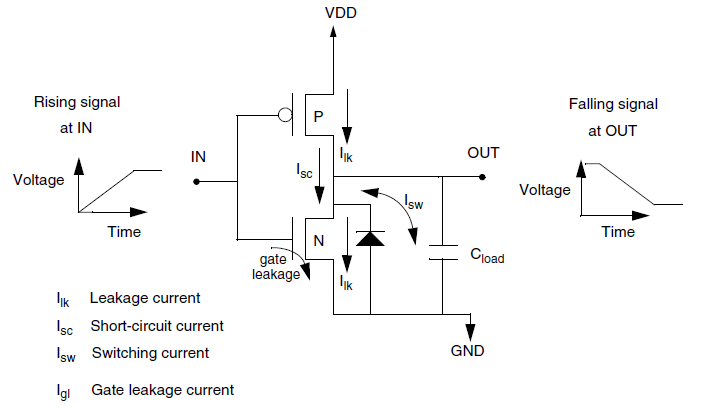
\includegraphics[width=\textwidth]{prime_time_power}
	\caption[Komponenten der Leistungsaufnahme]{Komponenten der Leistungsaufnahme \cite{primeTime2016}}
	\label{fig:prime_time_power}
\end{figure}
Mithilfe dieses Evalutionsablaufes sind die in diesem Kapitel evaluierten Ergebnisse entstanden.
\section{Testprogramme}
Um den Einfluss der Register-Adressen besser verstehen zu können wurden Assemblerprogramme entwickelt, die den Einfluss von Target-, Source1- und Source2-Registern untersuchen. Hierbei sind die Testfälle nach Komplexität gestaffelt. In den folgenden Kapiteln wird nun auf die Ergebnisse der einzelnen Programme und deren Erkenntnisse eingegangen.
\subsection{Empirische Tests}
\label{cap:empirischeTests}
Um die aufgestellte Annahme, dass sich die Verlustleistung proportional zur Hamming-Distanz verhält, zu bestätigen, wurden zu Beginn Assemblerprogramme entworfen, die nur mit physikalischen bzw. festen Registern arbeiten.
Außerdem wurden vorerst der Best- und Worst-Case untersucht, um das maximale Optimierungspotenial zu ermitteln. Das Programm durchläuft dabei alle Möglichkeiten der Adress-Port-Zuweisung. Es testet zum einen die Register-Allokation und die damit verbundene Hamming-Distanz-Berechnung, zum anderen werden alle Einflüsse der Register-Adressierung ermittelt. Da der Prozessor zwei Register-Files mit jeweils zwei Write- und vier Read-Ports aufweist, bestehen für die Target-Register vier und für die Source-Register 16 Möglichkeiten der Portzuweisung (siehe Tabelle \ref{lese-port} sowie \ref{fig::schreib-port}). Dabei sind X2-Operationen ausgenommen. Im Worst-Case werden die Register so adressiert, dass die maximale Hamming-Distanz entsteht. Dabei wechseln die Adressen von Null auf 31, welches der maximalen Hamming-Distanz von fünf entspricht. Damit keine Einflüsse durch Scheduling oder Daten entstehen, wurden Instruktionen manuell geschedult und den einzelnen Issue-Slots zugewiesen. Somit ist die Anordnung der Assemblerbefehle für jeden Testfall identisch und der Einfluss ist demzufolge entkoppelt. Im Falle der Datenabhängigkeiten werden alle Register mit einer Null initialisiert und im Anschluss nicht verändert. Dadurch werden alle Instruktionen mit den selben Daten ausgeführt und somit besteht keine Abhängigkeit der Daten mehr.
Für den Fall des Best-Case wird die Adresse nicht verändert und immer auf die Adresse Null gelesen sowie geschrieben.
Das Power-Analyse-Tool zeigt nach dem Ausführen des Workflows (Abbildung \ref{fig:flow_power_analyse}) eine Übersicht über die Leistungsaufnahme des Prozessors an. Hierbei wird die Leistung in Internal-, Switching- und Leakage-Leistung aufgeteilt (siehe Abbildung \ref{fig:best_power_hierarchy}). Die Leakage-Power wird mit der jeweiligen Transistor-Konfigurationen und den anliegenden Spannungen berechnet. Bei der Leakage-Leistung handelt es sich um eine statische Verlustleistung. Internal- und Switching-Leistung sind hingegen dynamische Verlustleistungen, die von den Schaltvorgängen beeinflusst werden. Die Internal-Leistung inkludiert alle Leistungen, die in einer Zelle durch das Laden von Kapazitäten verursachte werden. Dagegen werden in der Switching-Leistung die Verlustleistungen berücksichtigt, die durch das Laden von externen Lastkapazitäten verursacht werden.
Diese Leistungen werden hierarchisch nach den einzelnen Prozessor-Modulen aufgeschlüsselt. Die letzte Spalte des Reports zeigt die Aufteilung der Leistungsaufnahme in Prozent. Dabei ist zu erkennen, dass das Register-File (vrf\_inst) mit 65,2\% die größte Leistungsaufnahme im Prozessor aufweist.

\begin{figure}[H] 
	\centering
	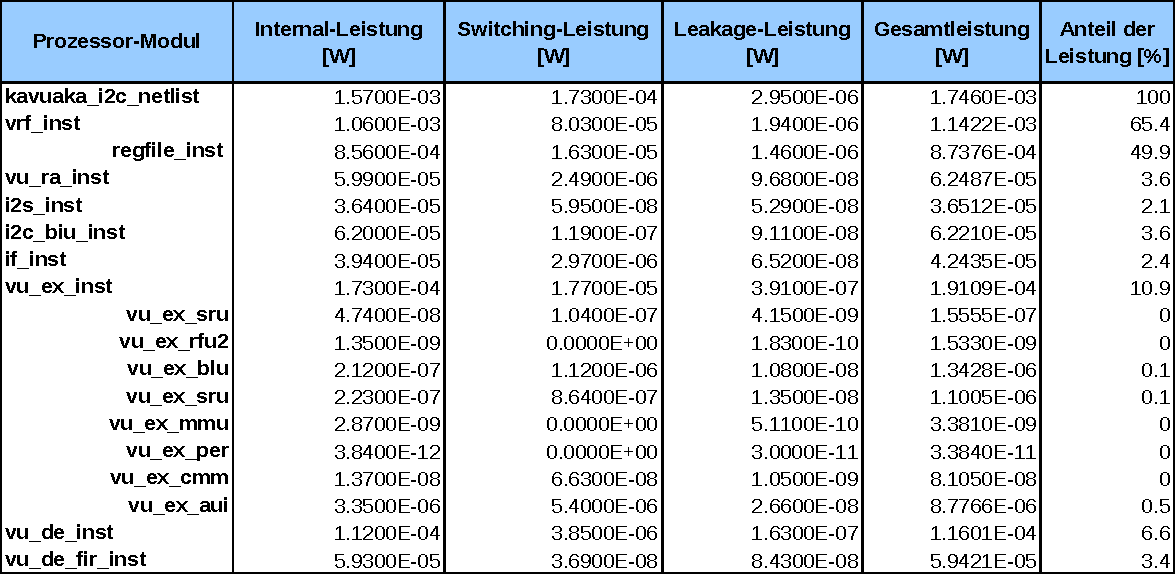
\includegraphics[width=\textwidth]{fig/best_hierarchy_report.pdf}
	\caption{Best-Case hierarchische Leistungsaufnahme}
	\label{fig:best_power_hierarchy}
\end{figure}

Aus beiden ermittelten Reports für den Worst- und Best-Case wurde die Tabelle (\ref{fig:best_powersave}.) erzeugt. Dabei sind die Einträge in Prozent angegeben und zeigen ein deutliches Einsparungspotential. Außerdem sind alle Prozente auf die Gesamtleistung der entsprechenden Spalte bezogen. Das Augenmerk sollte hierbei auf die Switching-Leistung des Register-Files gelegt werden, denn hier wurden die Veränderungen in der Adressierung erzeugt. Dabei ist deutlich zu erkennen, dass eine maximal Einsparung von 38,65\% zu erreichen ist. Dies zeigt sehr deutlich, dass die Adressierung der Register eine Auswirkung auf die Verlustleistung hat. In den anderen Modulen des Prozessors sind ebenfalls Verbesserungen zu erzielen. Das liegt vor allem daran, dass die Register-Adressen ebenfalls in diesen angelegt sind. Bei der Execution-Stage ist keine Verbesserung zu erzielen, da dort nur die Daten der jeweiligen Instruktion anliegen. Die Verbesserung der internen Leistungsaufnahme kann damit begründet werden, dass die Adressen ebenfalls Einfluss auf die interne dynamische Verlustleistung haben.
Das Resultat der unterschiedlichen Adressierungen ist eine Gesamtverlustleistungseinsparung von 7,87\%.

\begin{figure}[H] 
	\centering
	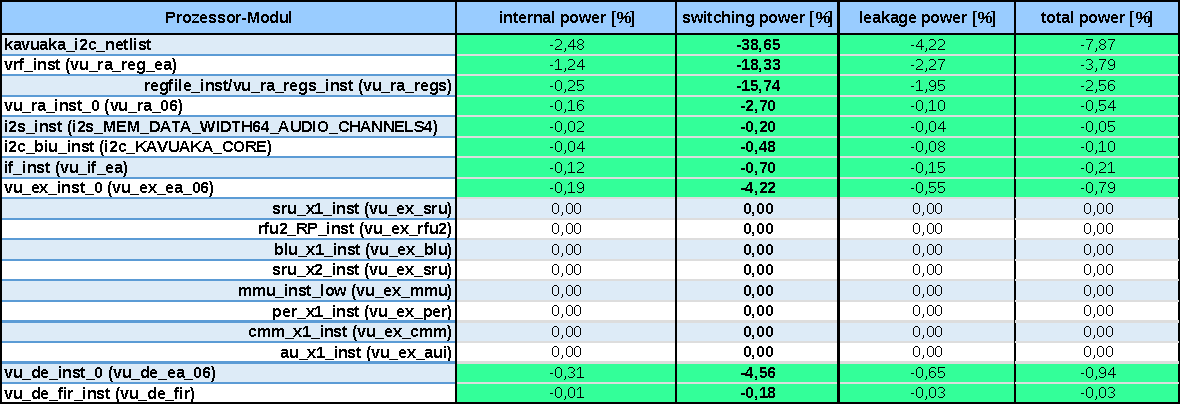
\includegraphics[width=\textwidth]{fig/best_worst_compare.pdf}
	\caption{Einsparungspotential Best-Worst-Case}
	\label{fig:best_powersave}
\end{figure}
\subsection{Synthetische Testprogramme}
Da nun gezeigt wurde, dass ein Zusammenhang zwischen Adressierung und Verlustleistung besteht, soll die Register-Allokation nun näher untersucht werden. Hierzu wurden synthetische Testfälle erstellt, welche mit unterschiedlichen Adressierungen, aber den selben Daten, arbeiten. Dabei wurden vorerst die Register einzeln betrachtet. Um die einzelnen Ergebnisse vergleichen zu können, wurden die Programme so entworfen, dass die Hamming-Distanzen für alle Testfälle identisch ausfallen. Das heißt, die Schaltaktivitäten in den Lese- sowie Schreibports sind identisch und die Leistungen können somit verglichen werden. Ein Beispiel für ein solches Testprogramm, welches den Einfluss der Target-Register testet, finden sie im Codebeispiel \ref{code:target_switching_test}. Um die Source-Register vom Test zu entkoppeln, wurden die Adressen der Register, die nicht untersucht werden sollten, nicht verändert. Dadurch entsteht keinerlei Schaltaktivität in den Adressleitungen. Gestartet wird die Berechnung der Hamming-Distanz immer mit der Adresse 0, da keine Aussage getroffen werden kann, welche Adresse in der letzten SLM zugewiesen wurde.

\begin{algorithm}[H]
	\begin{algorithmic}[1]
		\STATE {:0 \textbf {ADD} V0R2 V0R0 V1R0 \hspace{50pt}:1 \textbf {OR} V0R2 V0R0 V1R0}
		\STATE {:0 \textbf {ADD} V0R0 V0R0 V1R0 \hspace{50pt}:1 \textbf {OR} V1R2 V0R0 V1R0}
		\STATE {:0 \textbf {ADD} V1R0 V0R0 V1R0 \hspace{50pt}:1 \textbf {OR} V0R2 V0R0 V1R0}
		\STATE {:0 \textbf {ADD} V1R2 V0R0 V1R0 \hspace{50pt}:1 \textbf {OR} V1R2 V0R0 V1R0}
		\STATE {:0 \textbf {ADD} V0R0 V0R0 V1R0 \hspace{50pt}:1 \textbf {OR} V0R0 V0R0 V1R0}
		\STATE {:0 \textbf {ADD} V0R2 V0R0 V1R0 \hspace{50pt}:1 \textbf {OR} V1R0 V0R0 V1R0}
		\STATE {:0 \textbf {ADD} V1R2 V0R0 V1R0 \hspace{50pt}:1 \textbf {OR} V0R0 V0R0 V1R0}
		\STATE {:0 \textbf {ADD} V1R0 V0R0 V1R0 \hspace{50pt}:1 \textbf {OR} V1R0 V0R0 V1R0}
		\caption{Codebeispiel Target-Register }
		\label{code:target_switching_test}
	\end{algorithmic}
\end{algorithm}

Dieser Test wurde für die Adressen Zwei, Fünf, 24, 25 ,27 und 31 ausgeführt. Außerdem wurden Target, Source 1 und Source 2 getestet. Die untenstehenden Schaubilder (\ref{fig:source0_power}., \ref{fig:source1_power}., \ref{fig:target0_power}. sowie \ref{fig:target1_power}.) zeigen hierbei der Schaltleistung der verschiedenen Testfälle. Es ist zu erkennen, dass die Schaltleistungen der Lese- sowie Schreibports linear mit der Hamming-Distanz steigen. Außerdem sind die Graphen der Source-Register nahezu identisch, was impliziert, dass die Adressen in den Lese-Ports eine identische Verlustleistung verursachen.\\

\begin{figure}[H]
	\centering
	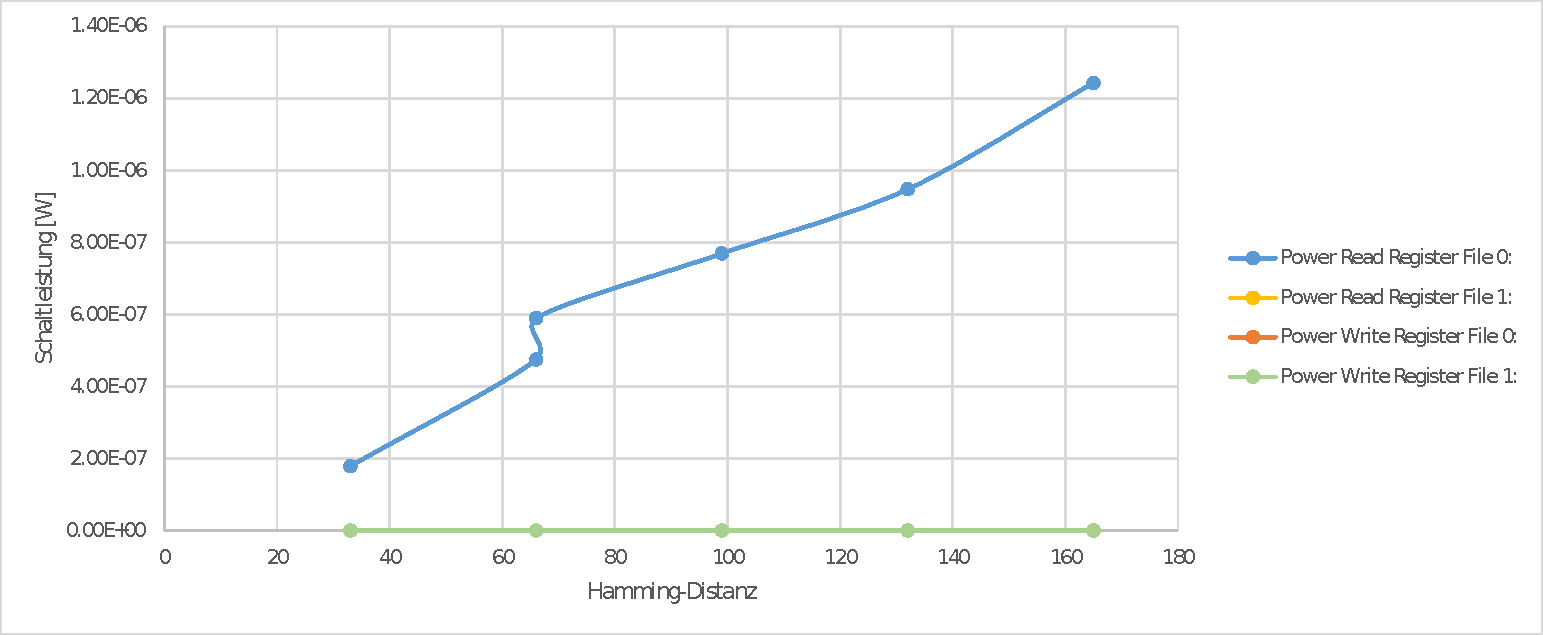
\includegraphics[width=\textwidth]{fig/source1_power.pdf}
	\caption{Schaltleistung Read Register File 0}
	\label{fig:source0_power}
\end{figure}
\begin{figure}[H]
	\centering
	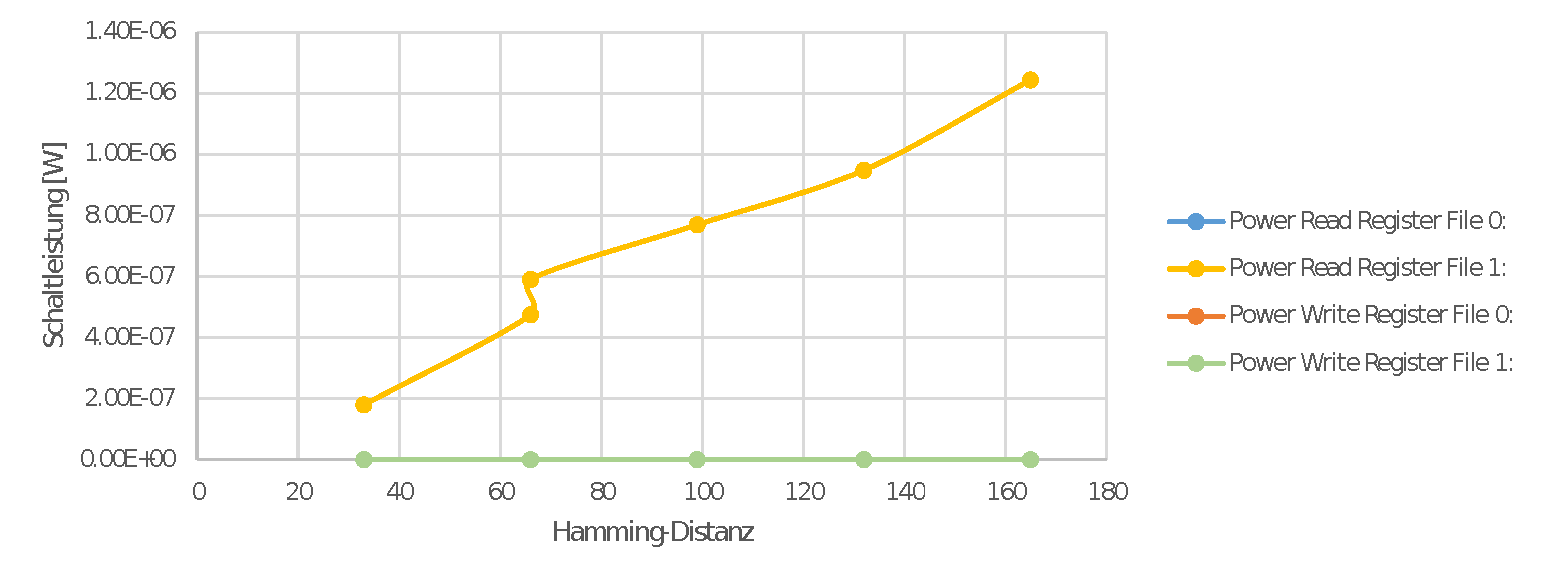
\includegraphics[width=\textwidth]{fig/source2_power.pdf}
	\caption{Schaltleistung Read Register File 1}
	\label{fig:source1_power}
\end{figure}
\begin{figure}[H]
	\centering
	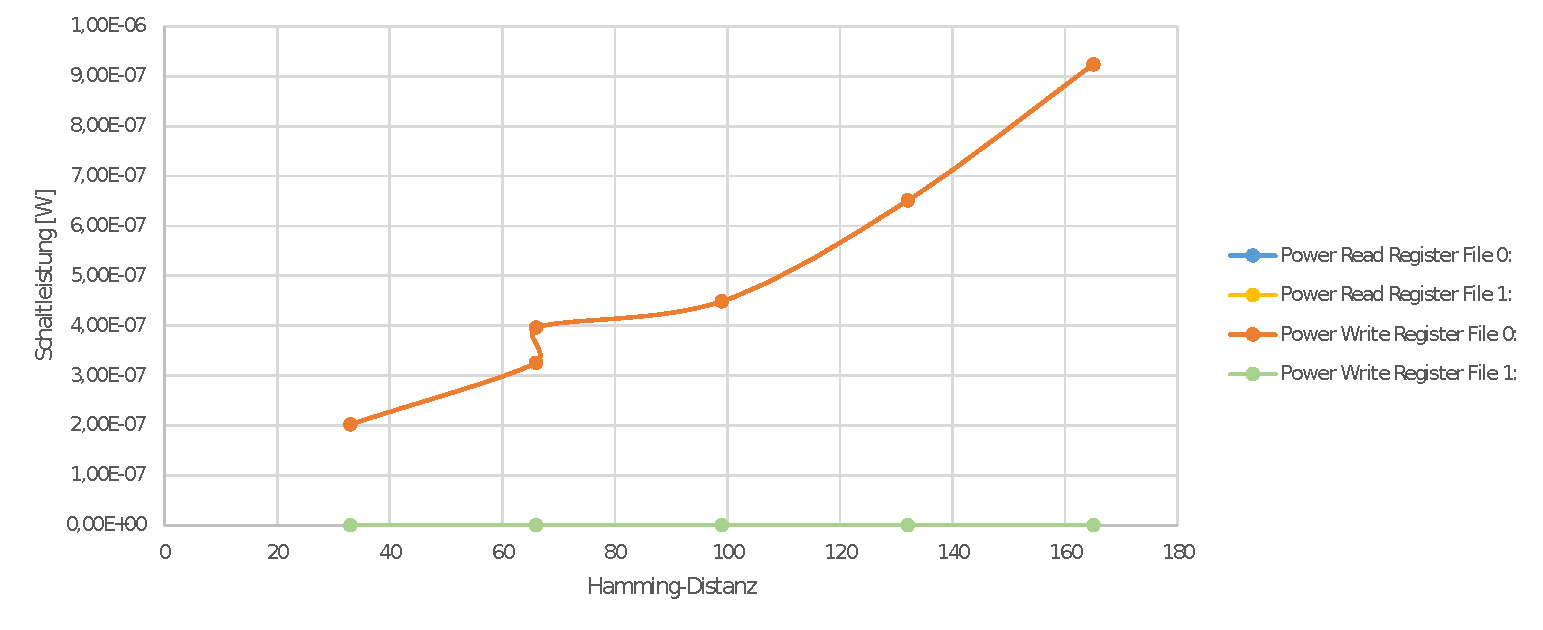
\includegraphics[width=\textwidth]{fig/register_eval_target_port0.pdf}
	\caption{Schaltleistung Write Register File 0}
	\label{fig:target0_power}
\end{figure}
\begin{figure}[H]
	\centering
	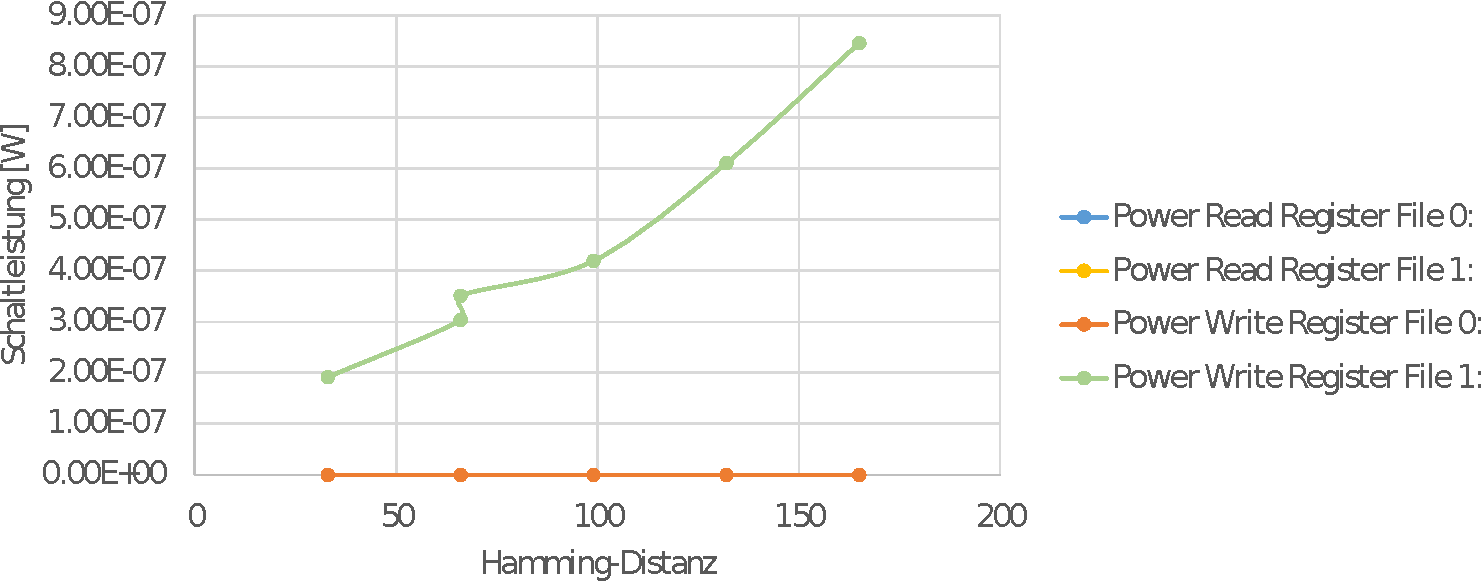
\includegraphics[width=\textwidth]{fig/register_eval_target_port1.pdf}
	\caption{Schaltleistung Write Register File 1}
	\label{fig:target1_power}
\end{figure}

Bei allen vier Graphen ist ein Sprung der Leistung bei einer Hamming-Distanz von 64 auffällig. Dieser lässt sich dadurch erklären, dass zwar die Hamming-Distanzen der Testfälle mit den Register-Adressen fünf und 24 identisch sind, aber unterschiedliche Adressleitungen verwendet werden, welche eine größere Lastkapazität aufweisen. Durch die höhere Lastkapazität wird automatisch auch einer größere Leistung benötigt. Dieses Phänomen wird in Kapitel \ref{cap:lastkapa} näher untersucht und erläutert.\\
Nach dem die Register nun getrennt voneinander betrachtet wurden und sich gezeigt hat, dass die Adressen ungefähr die selben Schaltleistungen in den Ports verursachen, soll nun das Verhalten beim gemeinsamen Schalten der Source- sowie Target-Register untersucht werden. Auch hierbei werden die Tests mit den selben Hamming-Distanzen für Lese- und Schreib-Ports ausgeführt. Das Schaubild \ref{fig:source_target_power}. zeigt auch hier, dass ein linearer Verlauf erkennbar ist.

\begin{figure}[H]
	\centering
	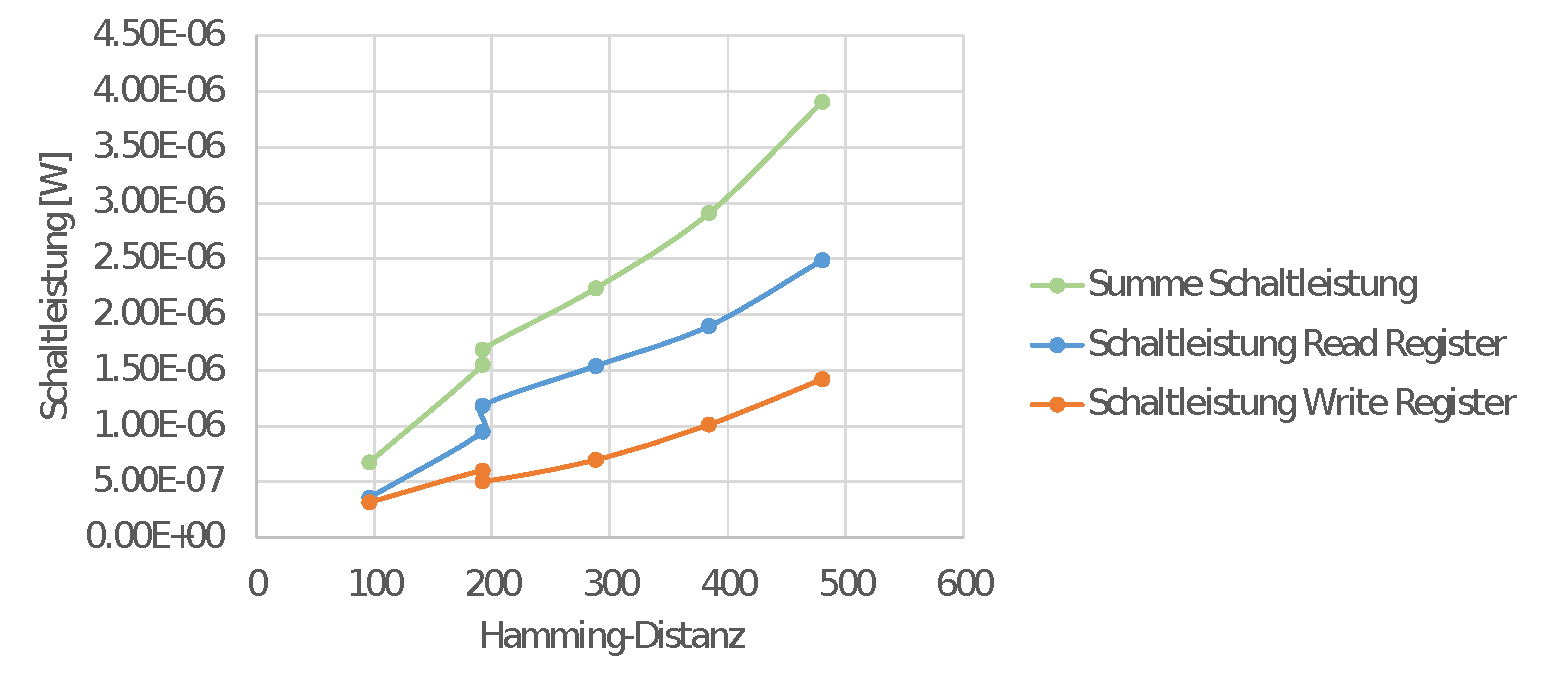
\includegraphics[width=\textwidth]{fig/source_target_power.pdf}
	\caption{Schaltleistung Read+Write Register}
	\label{fig:source_target_power}
\end{figure}

Außerdem zeigt Abbildung \ref{fig:total_power_source_target} die Gesamtleistung des Prozessors über der Hamming-Distanz. Auch hier ist eine deutliche Verbesserung erkennbar, welche sich ebenfalls linear zur Hamming-Distanz verhält.

\begin{figure}[H]
	\centering
	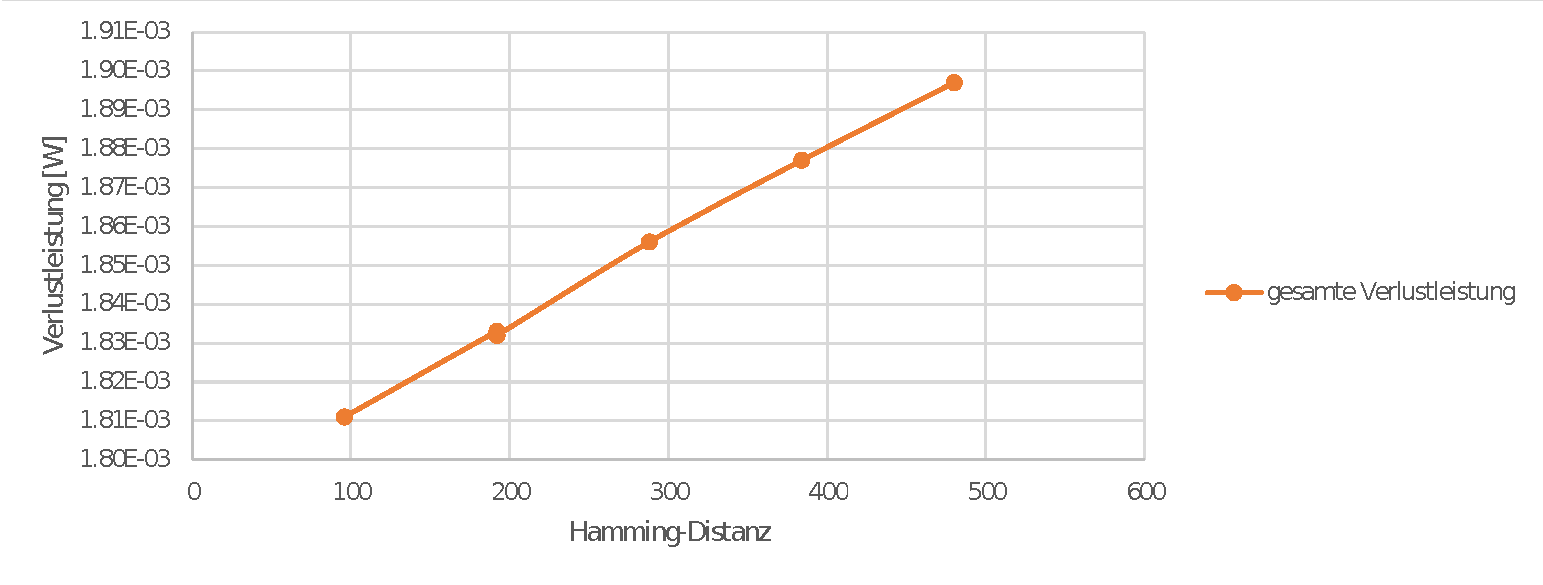
\includegraphics[width=\textwidth]{fig/total_power_source_target.pdf}
	\caption{gesamte Verlustleistung des Prozessors}
	\label{fig:total_power_source_target}
\end{figure}

Um nun ebenfalls den Einfluss der Daten auf die Verlustleistung zu ermitteln, wurden vorerst alle Register mit zufälligen Zahlen initialisiert und im Anschluss die oben beschriebenen Funktionen abgearbeitet. Diese Änderung verursacht einen Anstieg der Verlustleistung, jedoch ist zu untersuchen, ob die Einsparung durch die Adressierung feststellbar ist. Hierzu wurden die Testfälle mehrere Male durchlaufen, so dass die Werte aussagekräftig sind. Das untenstehende Schaubild \ref{fig:random_data_total_power} zeigt hierbei die Verläufe des Testfalls mit null initialisierten Daten in rot und mit Zufallszahlen befüllten Registern in blau. Es ist deutlich zu erkennen, dass trotz einer Abhängigkeit der Daten die Optimierung der Adressen feststellbar ist und die Verläufe sich ähneln.

\begin{figure}[H]
	\centering
	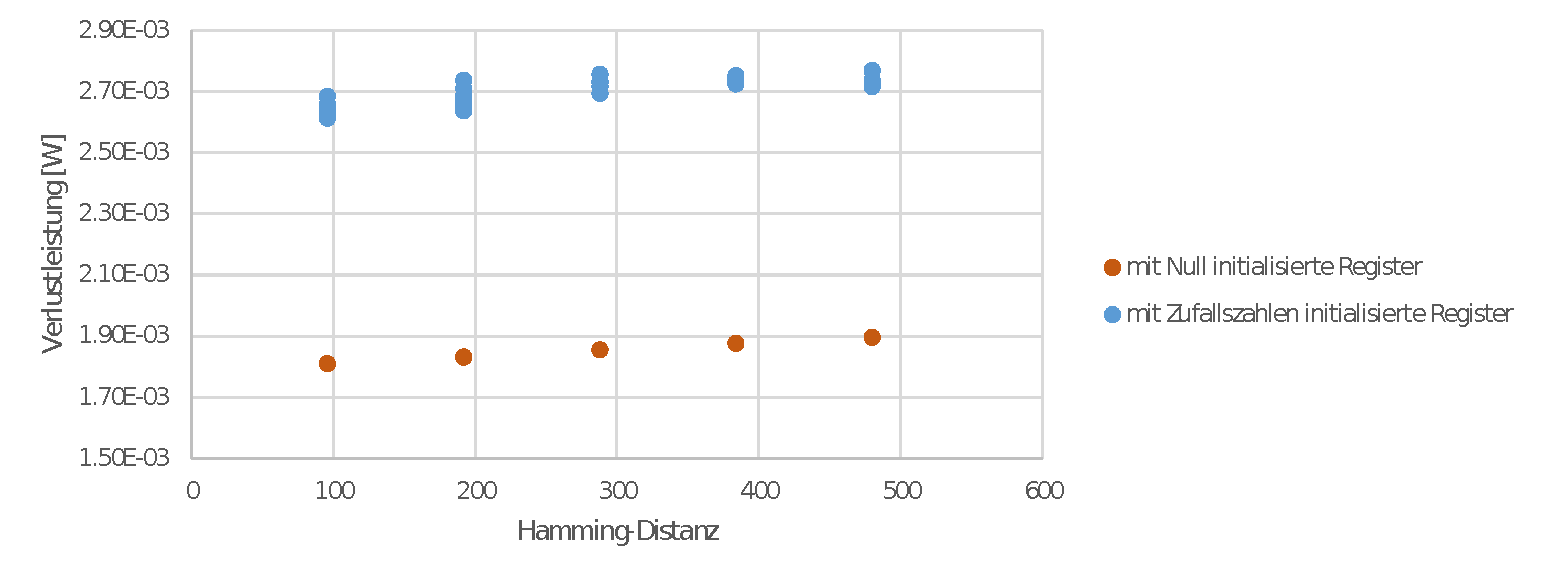
\includegraphics[width=\textwidth]{fig/random_data_total_power.pdf}
	\caption{Einfluss der Daten auf die gesamte Verlustleistung}
	\label{fig:random_data_total_power}
\end{figure}


\subsection{Heuristik}
\label{chap:eval_heuristik}
Da nun die Abhängigkeiten der Register-Adressierung zu der Verlustleistung gezeigt wurde, kann dieser Ansatz durch den Einsatz von virtuellen Registern ausgenutzt werden, um eine verbesserte Heuristik zu implementieren. Hierzu werden wie in Kapitel \ref{cap:empirischeTests}. Assemblerprogramme entworfen, welche manuell geschedult sind und die Register mit Null initialisiert werden. Der Unterschied zu den empirischen Testprogrammen liegt darin, dass nun ebenfalls virtuelle Register verwendet werden.
Dies hat zur Folge, dass die Register-Allokation eine geeignete Zuweisung finden muss und somit die Schaltaktivität der Adresse minimieren kann. Das Testprogramm belegt vorerst durch physikalische Adressierung eine gewisse Anzahl an Registern vor und blockiert diese somit für die Verwendung von virtuellen Register (siehe Abbildung \ref{fig:heuristik_eval}. - blau hinterlegte Felder).
Nachdem die Register-Files vorbelegt wurden, wird mit der Zuweisung von virtuellen Registern begonnen. Ab diesem Punkt ergeben sich Veränderungen in der Register-Allokation. Je nach gewähltem Verfahren, wird nach den optimalen physikalischen Registern mit unterschiedlichen Algorithmen gesucht. 

\begin{figure}[H] 
	\centering
	\includesvg[width=\textwidth]{heuristik_eval}
	\caption{Heuristik Evaluation}
	\label{fig:heuristik_eval}
\end{figure}
Das Schaubild \ref{fig:heuristik_eval} zeigt den Vergleich eines der implementierten Tesprogramme der alten zur neuen Heuristik. Die blockierten Register-Adressen sind blau hinterlegt, die von den Algorithmen ausgewählten Register-Adressen sind rot gekennzeichnet. Durch die beiden unterschiedlichen Verfahren ergibt sich ein Unterschied von 43 Schaltvorgängen in den Adress-Leitungen. Damit dieser in der Verlustleistung deutlicher zu erkennen ist, wird die Zuweisung der virtuelle Register 20 mal wiederholt. Dadurch ergibt sich ein Differenz der Hamming-Distanzen von 556, dies ist kein Vielfaches von 43, da durch das wiederholte Ausführen der Allokation die Zuweisung mit unterschiedlichen Adressen gestartet wird.
Damit der Zusammenhang von Verlustleistung zu Schaltaktivität zu erkennen ist, wurden sechs solcher Testfälle mit unterschiedlichen Hamming-Distanzen entwickelt. Hierbei variieren die Distanzen im Bereich zwischen 1173 und 2046 für die alte Heuristik. Diese werden von der neuen Heuristik auf einen Hamming-Distanz-Bereich von 794 bis 1165 optimiert.
Die Abbildung \ref{fig:schaltleistung_heuristic}. zeigt den Verlauf der Schaltleistung an den Adressports gegenüber der Hamming-Distanz. Es ist auch hier ein linearer Verlauf der Leistung zu erkennen. Die Verschlechterung der Schaltleistung trotz höherer Hamming-Distanz lässt sich mit unterschiedlichen Lastkapazitäten begründen. Durch eine Berücksichtigung dieser würde die Heuristik die Verlustleistung noch besser modellieren können. 
\begin{figure}[H]
	\centering
	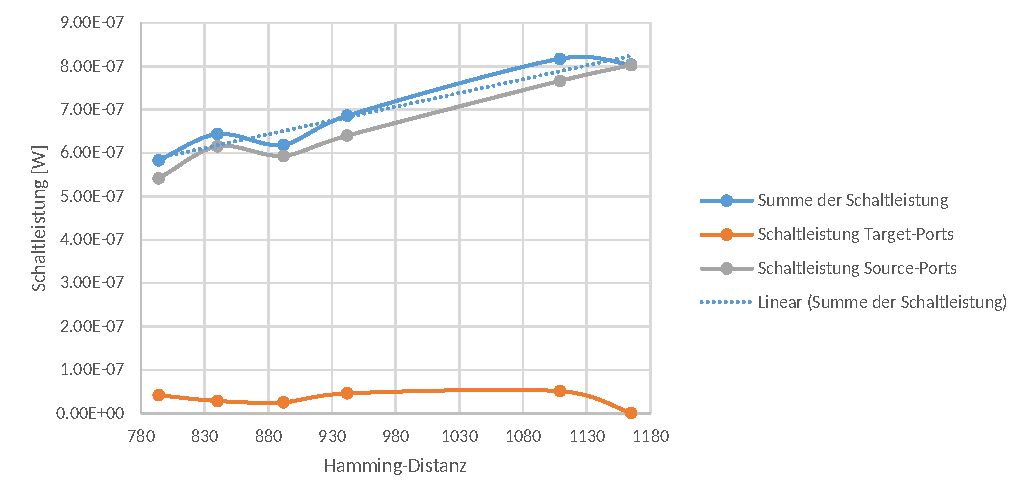
\includegraphics[width=\textwidth]{fig/schaltleistung_heuristic.pdf}
	\caption{Schaltleistung Target- und Source-Adressports}
	\label{fig:schaltleistung_heuristic}
\end{figure}

Nach der Betrachtung der Schaltleistung für die neue Heuristik zeigt Schaubild \ref{fig:heuristic_schaltleistung_alt_neu}. den Verlauf der Schaltleistungen an den Register-Ports gegenüber der Hamming-Distanz. 

\begin{figure}[H]
	\centering
	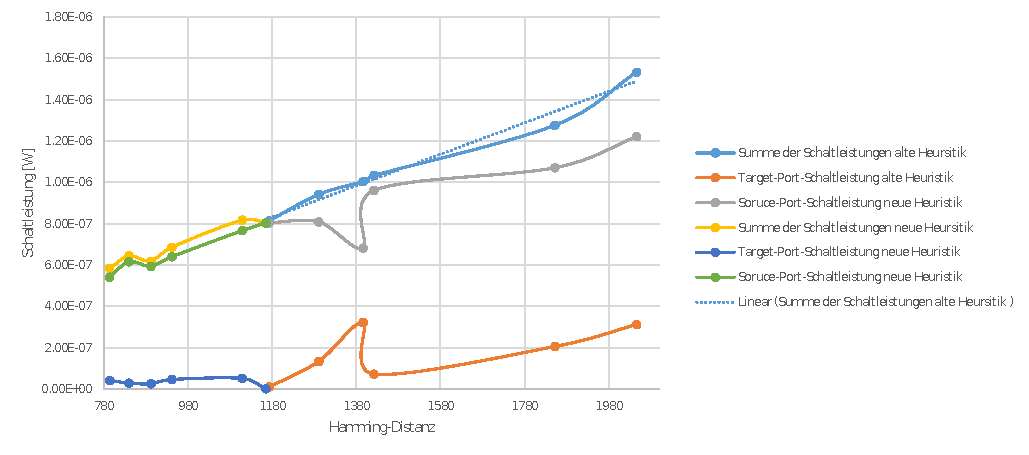
\includegraphics[width=\textwidth]{fig/heuristik_schaltleistung_alt_neu.pdf}
	\caption{Vergleich der Schaltleistungen von Target und Source-Ports}
	\label{fig:heuristic_schaltleistung_alt_neu}
\end{figure}

Dabei ist zu erkennen, das die neu implementierte Heuristik eine deutlich bessere Lösung findet. Im Schaubild sind die Daten nach ihrer Hamming-Distanz sortiert. Demnach kann kein Vergleich der einzelnen Datenpunkte zwischen den beiden Heuristik gezogen werden. 
Die Evaluation der Heuristik zeigt, dass für die entwickelten synthetischen Testfälle die neue Heuristik eine durchschnittliche Verbesserung der Schaltleistung der Adressports von 37,40\% erzielt werden kann.\\
Die Tabelle \ref{fig:compare_power_heuristic}. zeigt die Optimierung der Verlustleistung eines Testfalls, dabei sind die einzelnen Module des Prozessors gegenüber der alten Heuristik aufgeschlüsselt. Alle Werte sind in Prozent angegeben und beziehen sich auf die Gesamtleistungen der Spalten. Auch hier ist zu erkennen das deutliche Einsparungen in den Register-Files generiert werden konnten. Dabei wurde die Schaltleistung im Register-File gegenüber der alten Heuristik um 8,53\% verbessert. Die gesamte Verlustleistung wurde um 2,56\% optimiert. 

\begin{figure}[H]
	\centering
	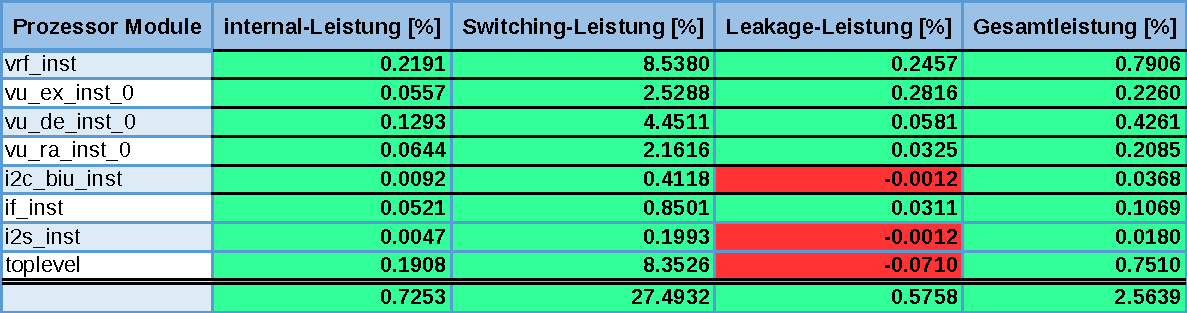
\includegraphics[width=\textwidth]{fig/compare_power_heuristic.pdf}
	\caption{Prozentuale Verbesserung der Verlustleistung- alte zu neue Heuristik}
	\label{fig:compare_power_heuristic}
\end{figure}


\subsection{Evaluation des genetischen Algorithmus}
Da die Heuristik, wie bereits in Kapitel \ref{sec:genetischerAlgorithmus} erwähnt, nur die Target-Register auf Schaltaktivität minimiert werden, wird nun die Verbesserung der Verlustleistung durch zusätzliches optimieren der Source-Register untersucht.
Bei der Evaluation wurde ein genetischer Algorithmus verwendet, der mit einer Heuristik eine Startpopulation berechnet, um eine schnelle Konvergenz gegen ein Minimum zu garantieren. Außerdem wird die Mutationswahrscheinlichkeit dynamisch angepasst. Als Fitness-Funktion wird die Multiplikation aus Hamming-Distanz und Lastkapazität gewählt. 
Um den Optimierungsgrad gegenüber der alten und neuen Heuristik vergleichen zu können, wurde der genetische Algorithmus mit den selben synthetischen Testprogrammen wie in Kapitel \ref{chap:eval_heuristik} getestet.
Da der genetische Algorithmus zufallsgesteuert ist, variieren die Ergebnisse stark. Um dennoch eine Aussage über die Verbesserung gegenüber der Heuristik treffen zu können, wurden die Testfälle mehrmals ausgeführt. Das Schaubild  \ref{fig:schaltleistung_genetic_heuristik} zeigt, wie stark die Ergebnisse der gesamten Schaltleistung untereinander variieren. Dabei ist zu erkennen, dass der genetische Algorithmus in den meisten Fällen Verbesserung gegenüber der neuen Heuristik findet. In Testfall vier wurde vom genetischen Algorithmus keine Verbesserung gefunden, da die Heuristik für dieses Szenario bereits eine Lösung gefunden hat, die der Algorithmus in seiner Laufzeit nicht weiter minimieren konnte.  
\begin{figure}[H]
	\centering
	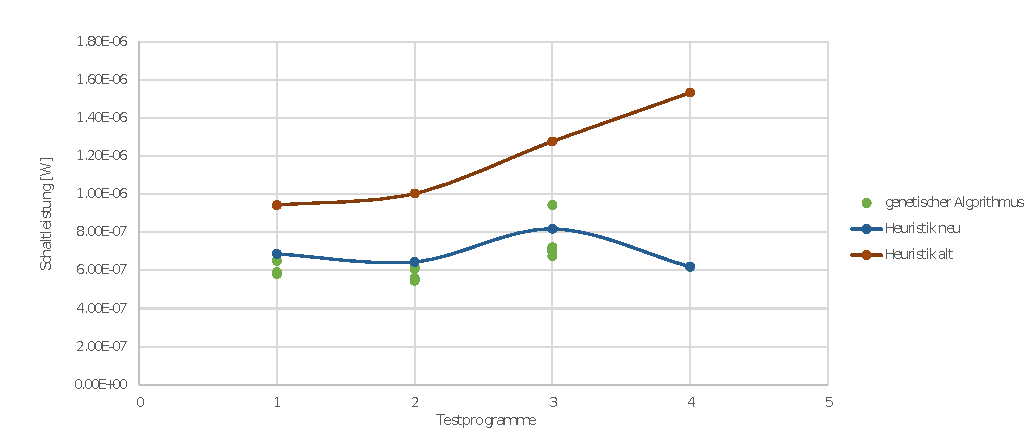
\includegraphics[width=\textwidth]{fig/schaltleistung_genetic_heuristik.pdf}
	\caption{Vergleich der Schaltleistungen für Heuristik und genetischer Algorithmus}
	\label{fig:schaltleistung_genetic_heuristik}
\end{figure}
Die durchschnittliche Verbesserung der Schaltleistung gegenüber der neuen Heuristik beträgt 7,83\% und 41,57\% im Vergleich zur alten Heuristik. Der genetische Algorithmus konnte im besten Fall eine Verbesserung von 17,38\% zur neuen Heuristik und 59,70\% zur alte Heuristik erreichen.\\
Das Schaubild \ref{fig:eval_genetic_total_power} veranschaulicht die Ergebnisse der Gesamtleistung des Prozessors. Dabei ist zu erkennen das die Leistung minimiert werden konnte, der genetische Algorithmus jedoch die Gesamtleistung nicht verbessern konnte. Die neue Heuristik konnte im durchschnitt eine Verbesserung der Verlustleistung von 1,82\% erreichen, im Gegensatz hierzu konnte der genetische die Verlustleistung nur auf 1,62\% optimieren. Dies impliziert, dass die Gesamtleistung noch von anderen Parametern abhängen muss und die Fitness-Funktion an diese angepasst werden muss.

\begin{figure}[H]
	\centering
	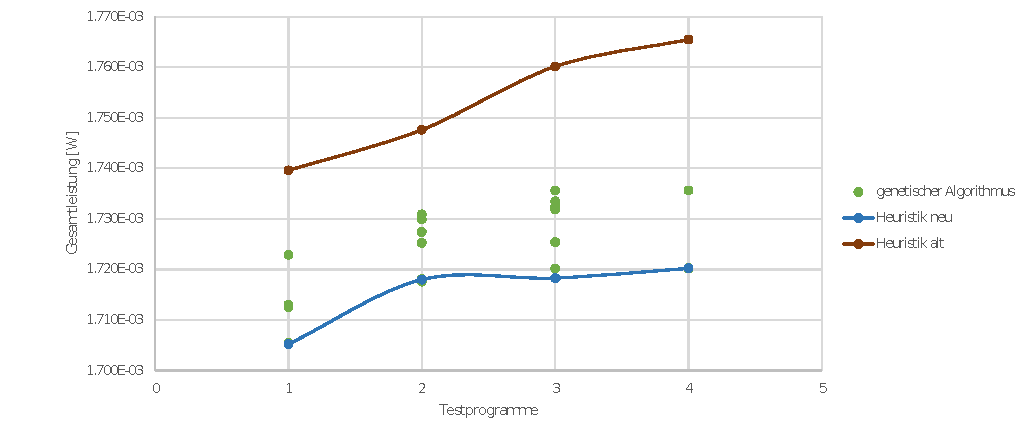
\includegraphics[width=\textwidth]{fig/gesamtleistung_genetik_heuristik.pdf}
	\caption{Gesamtverlustleistung genetischer Algorithmus vs. Heuristik}
	\label{fig:eval_genetic_total_power}
\end{figure}

Die komplette Einsparung fällt relativ gering aus, jedoch ist hervorzuheben, dass diese Optimierung komplett \glqq kostenfrei \grqq und ohne Veränderung der Hardware erzielt werden kann.
%Im unten stehenden Schaubild XXX wird der Mittelwert der Testfälle gegenüber der alten Heuristik veranschaulicht. 
%
%Mittelwert genetischer Algo gegenüber alter heuristik

Auch hier zeigt ein prozentualer Vergleich der Verlustleistungen des kompletten Prozessors eine Verbesserung der Schaltleistung in den Register-Files. In diesem Fall wird die beste Lösung des genetischen Algorithmus mit der alten Heuristik verglichen. Die Tabelle zeigt eine Verbesserung der Schaltleistung des Gesamten Prozessors um 7,78\%. Die Verlustleistung, die durch die Leakage-Ströme verursacht wurde, ist um zwei bzw. drei Zehnerpotenzen kleiner als die Verlustleistungen die durch die Schaltvorgänge hervorgerufen wird. Aus diesem Grund werden diese vernachlässigt. 
Die prozentuale Veränderung der Internal-Leistung liegt im sehr niedrigen Prozentbereich und wird ebenfalls nicht weiter berücksichtigt. 

\begin{figure}[H]
	\centering
	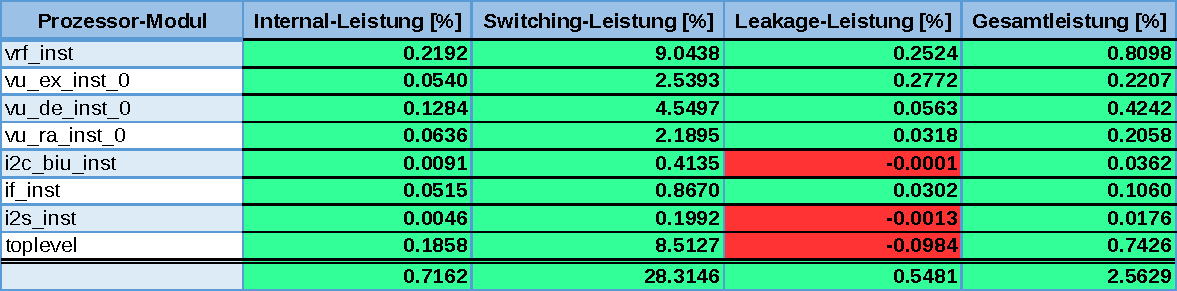
\includegraphics[width=\textwidth]{fig/power_percent_genetic.pdf}
	\caption{Prozentuale Verbesserung der Verlustleistung}
	\label{fig:power_percent_genetic}
\end{figure}

Die Schaubilder \ref{fig:totalpower_old}, \ref{fig:totalpower_new} sowie \ref{fig:totalpower_genetic} zeigen den Verlauf der Gesamtleistung des Prozessors gegenüber der Hamming-Distanz. Diese zeigen das Verhalten der Gesamtleistung und den Zusammenhang mit der Schaltaktivitäten der Adressports.

\begin{figure}[H]
	\centering
	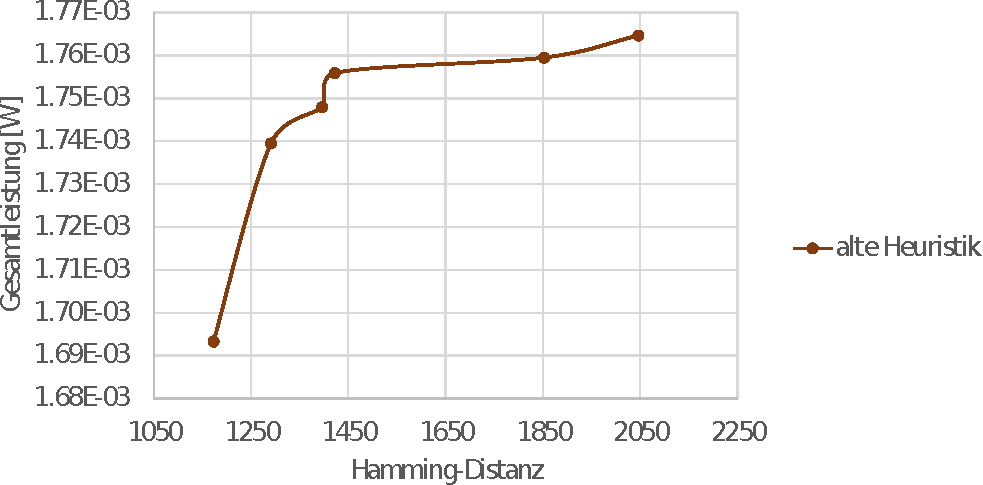
\includegraphics[width=\textwidth]{fig/totalpower_old.pdf}
	\caption{Verlauf der Gesamtleistung alte Heuristik }
	\label{fig:totalpower_old}
\end{figure}

\begin{figure}[H]
	\centering
	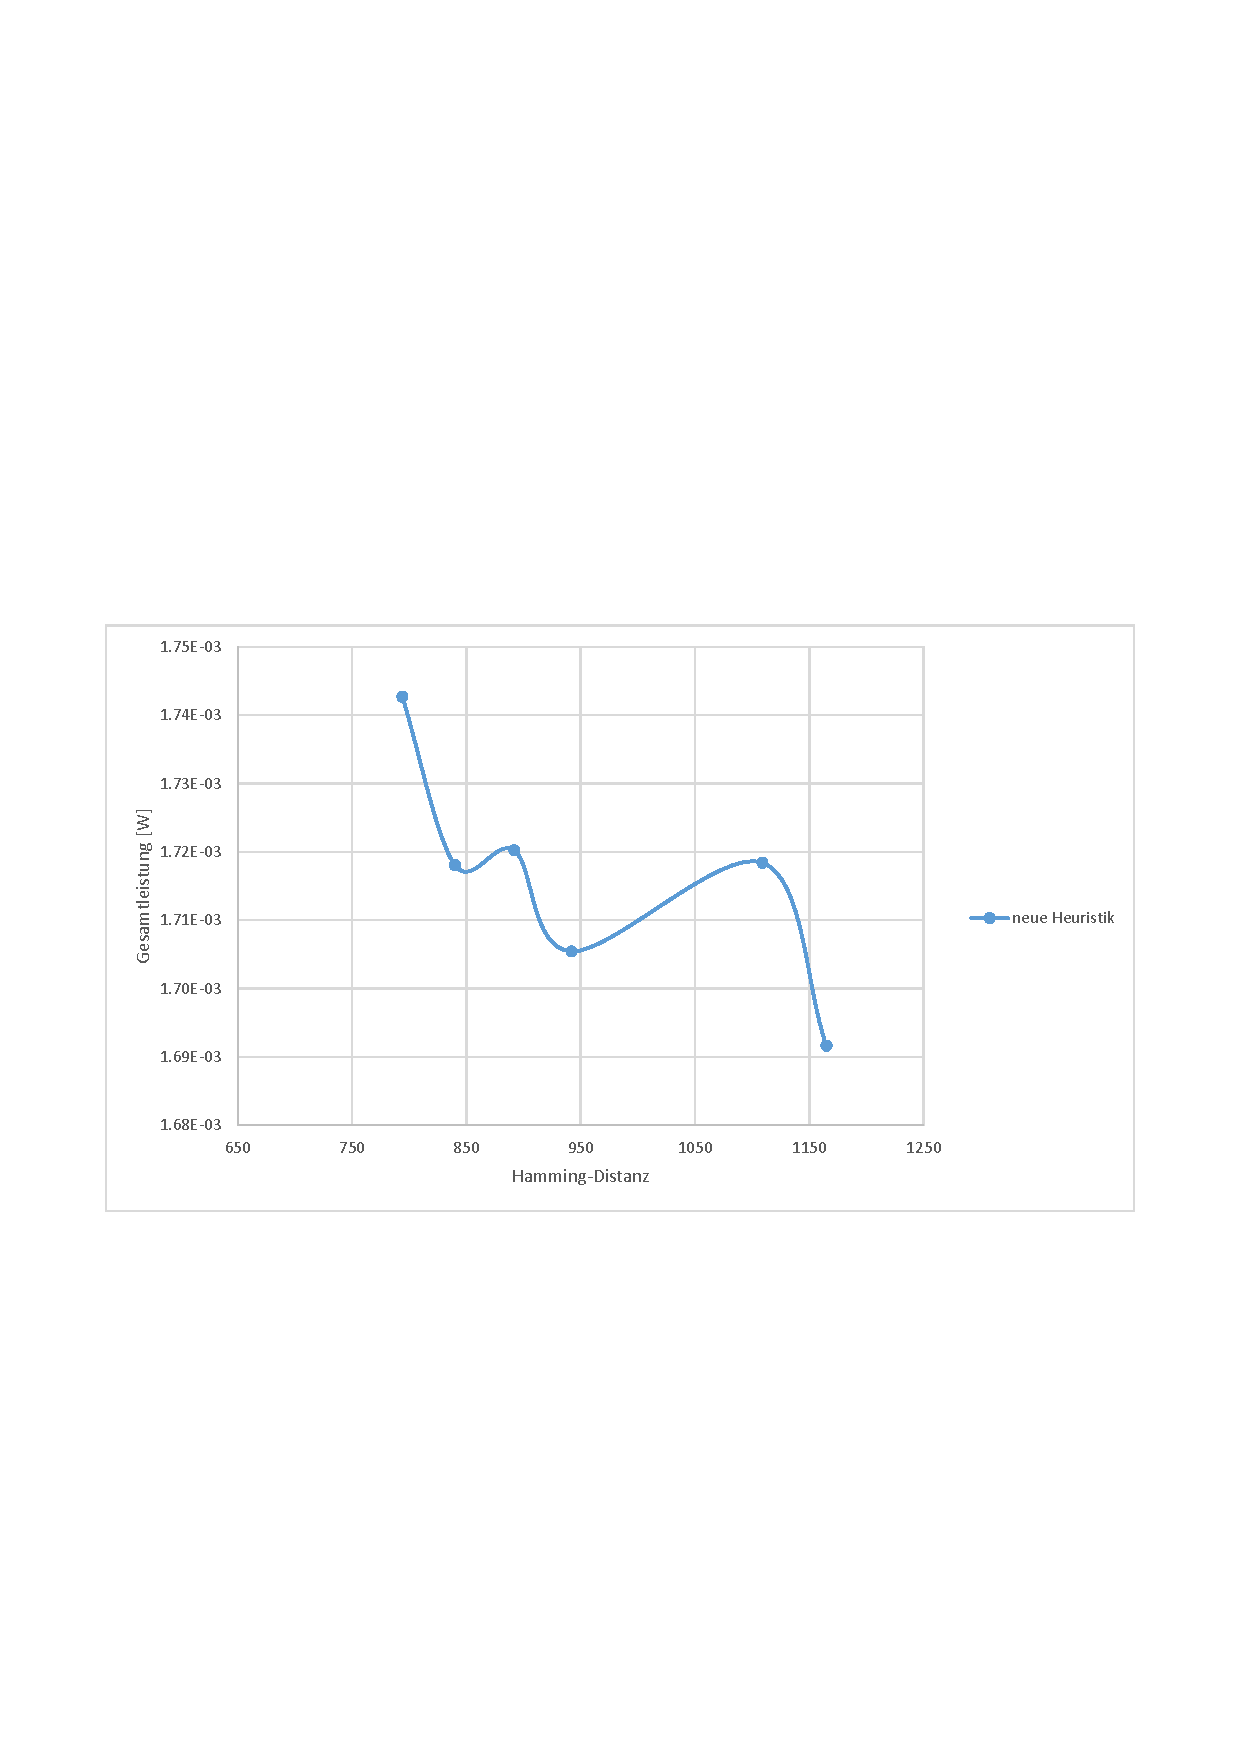
\includegraphics[width=\textwidth]{fig/totalpower_new.pdf}
	\caption{Verlauf der Gesamtleistung neue Heuristik}
	\label{fig:totalpower_new}
\end{figure}

\begin{figure}[H]
	\centering
	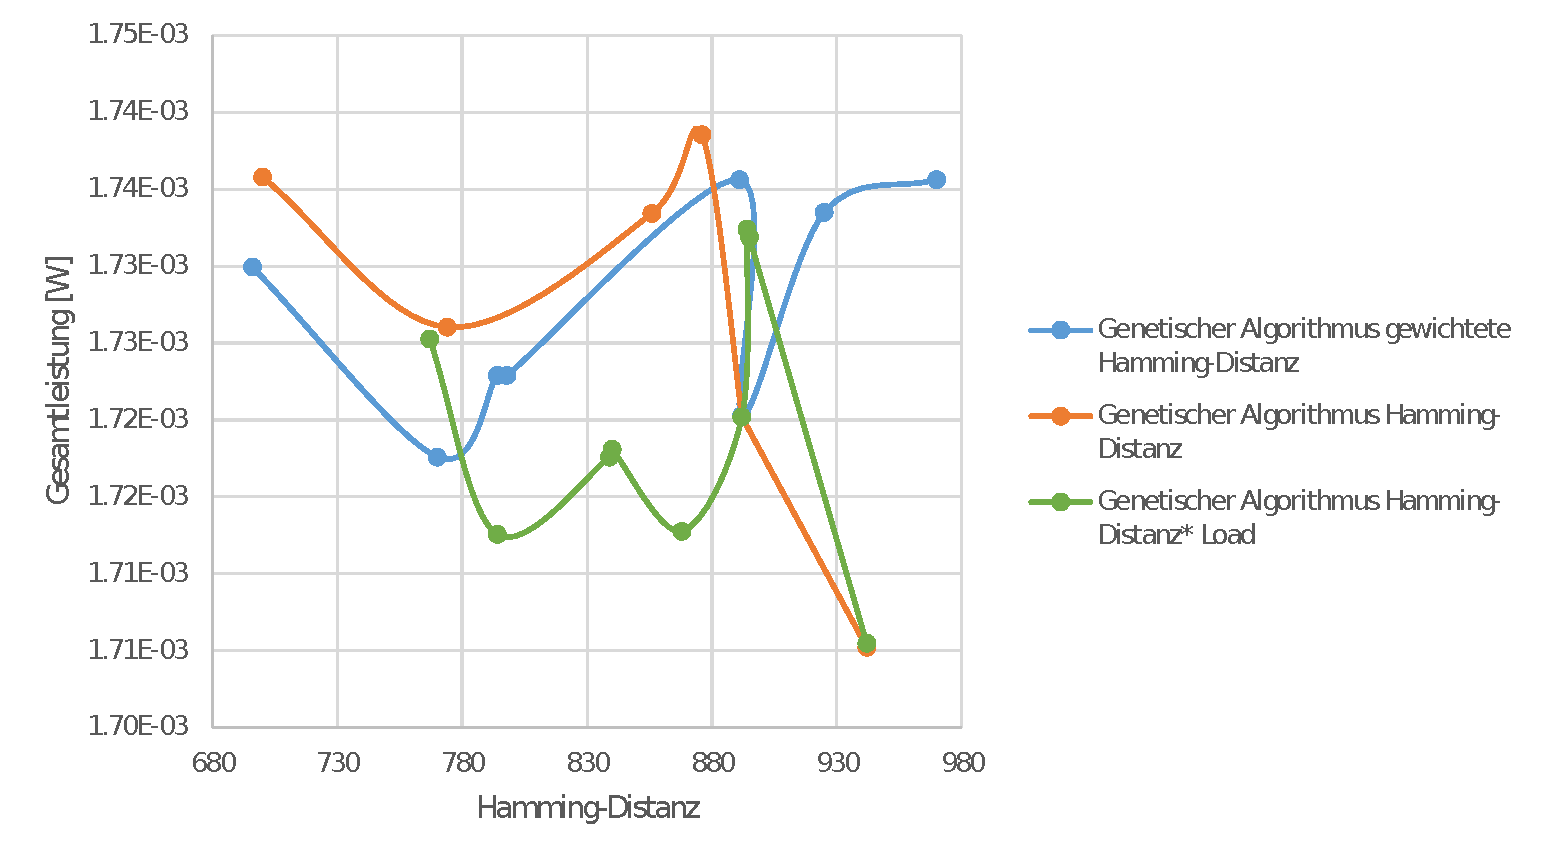
\includegraphics[width=\textwidth]{fig/totalpower_genetic.pdf}
	\caption{Verlauf der Gesamtleistung genetischer Algorithmus}
	\label{fig:totalpower_genetic}
\end{figure}

Bei der Gesamtleistung für die neuen Heuristik ist auffällig, dass die Leistung mit steigender Hamming-Distanz fällt. Das selbe Verhalten ist für den genetischen Algorithmus erkennbar. Im Gegensatz hierzu zeigt die alte Heuristik mit der Hamming-Distanz an. Dieses Phänomen muss näher untersucht werden, was jedoch den Umfang dieser Arbeit übersteigt.

\section{Hörgerätealgorithmen}
\label{sec:testprogamme}
Um den implementierten Code zu testen und eine reale Einsparung der Verlustleistungsreduktion zu ermitteln, wurden die folgenden Hörgerätealgorithmen verwendet. Dabei handelt es sich um die Programme die eine häufig Anwendung in Hörgerät-Prozessoren finden.

\subsection{Emulated Floating Point}
\label{chap:emulated_floating_point}
Da der verwendete Prozessor keine Gleitkommavariablen unterstützt, besteht eine softwarebasierte Methode der diese emuliert. Dabei wird eine Gleitkommazahl als zwei Subworte deklariert, zum einen der Signifikant $T$ und zum anderen der Exponent $E$. Mit Hilfe dieser kann eine Gleitkommazahl $f$ nach Formel \ref{eq:emulated_floating_point} berechnet werden.
\begin{equation}
f = T *2^E
\label{eq:emulated_floating_point}
\end{equation}
Beide Variablen $ T,E$ können als Subwort im Register gespeichert werden. Dabei können diese an eine beliebige Adresse des Registers stehen. Aus diesem Grund werden hierfür zwei virtuelle Register verwendet. Diese Emulation ist besonders geeignet für SIMD-Architekturen, bei der eine Gleitkommaberechnung ohne Aufschlüsseln der Variablen errechnet werden kann. Dadurch ist diese Art von Gleitkommaberechnung äußerst performant.
Wenn nun ein Algorithmus mit Gleitkommazahlen rechnet, werden viele temporäre Zwischenwerte berechnet, welches den Algorithmus prädestiniert für eine Adressoptimierung macht und aus diesem Grund Algorithmen verwendet werden, die mit diesen arbeiten. \cite{gerlach2016efficient}

\subsection{Filter und FFT mit emulated floating point}
Im folgenden wird die Verlustleistung der beiden Algorithmen zur Fast Fourier Transformation und zu einem Frequenzfilter analysiert. Die beiden Abbildungen \ref{fig:fft_vergleich_heuristik} und \ref{fig:fft_vergleich_genetisch} zeigen die Einsparungen die durch die neue Heursistik und den genetischen Algorithmus erreicht wurden.

\begin{figure}[H]
	\centering
	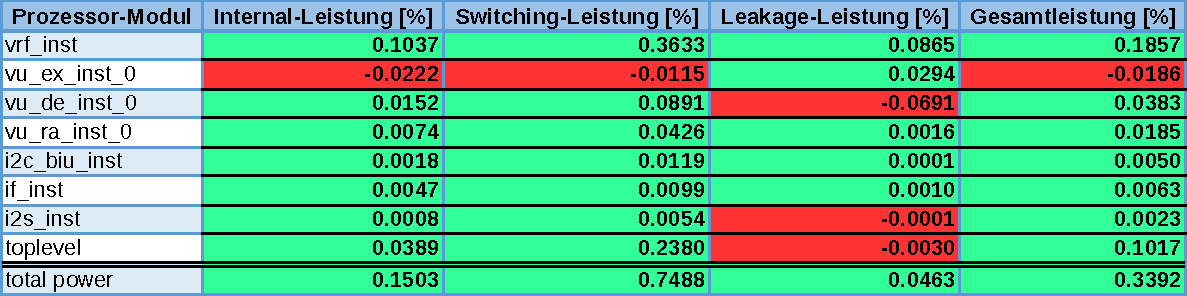
\includegraphics[width=\textwidth]{fig/fft_vergleich_heuristik.pdf}
	\caption{Gesamtleistungseinsparung FFT Heuristik}
	\label{fig:fft_vergleich_heuristik}
\end{figure}
\begin{figure}[H]
	\centering
	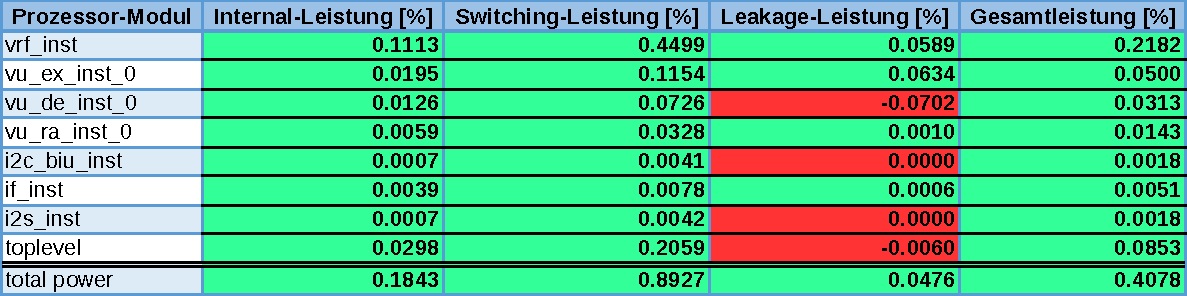
\includegraphics[width=\textwidth]{fig/fft_vergleich_genetisch.pdf}
	\caption{Gesamtleistungseinsparung FFT genetischer Algorithmus}
	\label{fig:fft_vergleich_genetisch}
\end{figure}

Im Fall der FFT ist eine Optimierung der Verlustleistung um 0.3392\% mit der Heuristik und um 0,4078\% mit dem genetischen Algorithmus zu erreichen. Dabei ist anzumerken, dass die Problemstellung der FFT mit nahe zu 8000 Instruktionen groß ausfällt und der genetische Algorithmus nur geringe Verbesserungen finden konnte. Durch ein längere Testdauer sollte es dem genetischen Algorithmus jedoch möglich sein weitere Verbesserungen zu finden.

%\subsection{Filter emulated floating Point}Der Filter mit Gleitkommazahl-Berechnung konnte hingegen eine Einsprung von XXX\% erzielen



%\subsection{Beamforming}
%Der Beamforming-Algorithmus wird eingesetzt um eine Positionsbestimmung von Schallwellen im Raum durchzuführen und somit eine Ein- bzw Ausblendung von verschiedenen Geräuschen zu gewährleisten und so das Hörerlebnis zu steigern. 

 


\section{Einfluss der Register-Daten auf die Verlustleistung}
In Kapitel \ref{cap:empirischeTests} wurde bereits der Einfluss der Daten auf die Verlustleistung ermittelt. Da sich nun jedoch eine Verschlechterung der Register-File-Leistung bei besserer Adressierung in den realen Testfällen ergibt wurden die Datenabhängigkeit nochmals überprüft. Dabei ergab sich, dass auf Grund des Verhalten des Adress-Decoders eine Veränderung der Daten verursacht wird. Da die Adressen über einen Adress-Decoder decodiert werden müssen und dieser nicht direkt alle Bits auf einmal umschalten kann, liegen kurze Zeit, Daten aus anderen Adressen an den Daten-Leitungen an. Dies Verursacht dort eine Schaltleistung welches die Verbesserung durch die Adressierung aufhebt.
%Um dieses Verhalten und die Funktion des Decoders besser nachzuvollziehen wurden nun weitere Testfälle generiert. Diese befüllen wie in Kapitel \ref{cap:empirischeTests} alle Register mit zufälligen Daten. Der unterschied liegt jedoch darin, dass die Instruktionen in allen Testfällen mit den selben Zufallsdaten arbeiten, so dass immer die selben Daten in die entsprechenden Register geschrieben werden.
%
%Hierbei war zu erkennen, 

\section{Einfluss der Lastkapazität  auf die Verlustleistung}
 \label{cap:lastkapa}
Wie bereits in Kapitel \ref{cap:empirischeTests} erwähnt, besteht eine Abhängigkeit zwischen Lastkapazität und Verlustleistung. Dies lässt sich auf die Formel der dynamischen Verlustleistung zurückführen \ref{eq:dynVerlustleistung}, laut dieser steigt die Verlustleistung linear mit der Lastkapazität.
Das untenstehende Schaubild \ref{fig:read_port_mux} zeigt, wie die Daten aus den Registern an die Read-Ports angelegt werden. Hierbei ist jedes Bit der Register-Adresse für das Schalten eines Multiplexers zuständig. Besteht nun der Fall, dass ein Register mit einer Adresse von 31 ausgelesen werden soll, so müssen alle Multiplexer durchschalten. Dadurch werden die Daten des Registers an den Verwendeten Register-Port weitergeleitet. Wird im Gegensatz hierzu eine niedrige Adresse, beispielsweise Null, angefragt, so muss keiner der Multiplexer schalten. Das Signal liegt direkt an dem Read-Port an. Aus diesem Grund benötigen die oberen Adressleitungen mehr Verlustleistung da das Signal eine höhere Lastkapazität aufweist. Dies lässt sich ebenfalls in den Power-Reports nachvollziehen. Dort ist deutlich zu erkennen, dass die oberen Register-Adressen eine höhere Lastkapazität aufweisen. 
\begin{scriptsize}
	\begin{figure}[htbp] 
		\centering
		\includesvg[width=\textwidth]{Read-Port-Mux}
		\caption{Read-Port Multiplexer}
		\label{fig:read_port_mux}
	\end{figure}
\end{scriptsize}

Aus diesem Grund wurde die Fitness Funktion des Genetischen Algorithmus so angepasst, dass die Lastkapazität zusätzlich berücksichtigt wird.

\clearpage
\newpage
%
\chapter{Schlussfolgerung}
\label{chap:schlussfolgerung}
Das Ziel dieser Arbeit war es, durch einen genetischen Optimierungsalgorithmus eine Register-Allokation zu finden, welche die Verlustleistung des KAVUAKA-Prozessors minimiert. Es wurde zu Beginn die These aufgestellt, dass die Verlustleistung proportional mit der Schaltaktivität der Register-Adressleitungen steigt. Durch einen Vergleich des Best- und Worst-Case-Adressierung, wurde ein Optimierungspotential von 7,87\% für die Verlustleistung des gesamten Prozessors und 38,65\% für die Schaltleistung ermittelt. Dadurch konnte ein klarer Zusammenhang der Schaltaktivität und der Verlustleistung festgestellt werden. Um diesen Ansatz in der Register-Allokation umzusetzen, wurde zu Beginn ein Modell gewählt, dass den Freiheitsgrad von virtuellen Registern ausnutzt und diese so allokiert, dass die Schaltaktivität der Register-Adressierung minimiert wird. Mittels einer neu implementierten Heuristik wurde so mithilfe der Hamming-Distanz die Schaltaktivität der Target-Port-Adressen minimiert. Dabei wurden in den programmierten synthetischen Test eine Verlustleistungseinsparungen von 1,82\% für die Gesamtverlustleistung gegenüber der alten Implementierung ohne Schaltaktivitätsoptimierung erzielt.
Um die Schaltleistungen noch weiter zu minimieren und ebenfalls die Source-Port-Adressen in die Optimierung mit einzubinden, wurde ein genetischer Optimierungsalgorithmus implementiert. Dieser optimiert anhand der Hamming-Distanz gepaart mit der Lastkapazität als Fitness-Wert die Schaltaktivität im Multishared Register-File. Dabei hat die Evaluation, mittels synthetischen Tests gezeigt, dass die Parameter des Algorithmus an das jeweilige Problem angepasst werden muss und nicht pauschalisiert werden kann. Eine Startpopulationsberechnung durch eine Heuristik und dynamische Anpassung der Mutationswahrscheinlichkeit ist jedoch für alle Problemstellungen sinnvoll.
Durch den Einsatz des genetischen Algorithmus kann die Hamming-Distanz der Adressen minimiert werde, welches eine Minimierung der Schaltleistung der Adress-Ports von durchschnittlich 41,57\% mit sich führt.  
Die Evaluation hat gezeigt, dass dadurch eine geeignete Adressierung gefunden werden kann, die die dynamische Verlustleistung insbesondere in den Register-Files minimiert. Dabei liegt die Einsparung gegenüber der alten Implementierung bei 1,62\% und konnte keine weitere Verbesserung zur neuen Heuristik generieren.
Für die realen Testfälle des emulated-floation-point Filter sowie FFT sind Einsparungen von XXX\% zu erzielen. Dabei ist zu beachten, dass es zu Schaltaktivitäten der Daten auf Grund des Verhaltens der Adressdecoder kommt und diese eine Verschlechterung der Verlustleistungsergebnisse in den realen Testfällen erzeugen.
Die erzielten Einsparungen sind nicht sehr hoch, werden jedoch nur durch eine Veränderung der Software erreicht. Dadurch muss kein Abtausch zwischen Energieeffizienz und Chipfläche stattfinden, welches eine deutlicher Vorteil gegenüber anderen Ansätzen darstellt.
Außerdem wurde der Einfluss der Lastkapazität auf die Verlustleistung festgestellt und aufgezeigt. Durch eine Berücksichtigung dieser, kann die Leistung weiter optimiert werden.
Dadurch das, dass die Register-Allokation dem Scheduling untergeordnet ist, kann es zu sehr langen Berechnungszeiten kommen. Dies ist insbesondere der Fall, wenn für das Scheduling und die Register-Allokation ein genetischer Algorithmus gewählt wurde. Außerdem steht die Berechnungsdauer mit der Anzahl an virtuellen Registern bei der genetischen Register-Allokation in Korrelation. Da jedoch für die meisten Programme ein List-Scheduling ausreicht, kann der genetische Algorithmus für die Register-Allokation immer eingesetzt werden.\\
Weitere ausgiebige Testes und Optimierungen der Parameter des genetischen Algorithmus, können in Zukunft das Verhalten der Verlustleitung weiter an das Optimierungspotential angleichen und so den Energiebedarf weiter senken. Außerdem könnte durch den Einsatz von Clock-Gating eine weitere Funktion eingebaut werden, die es ermöglicht die Schaltaktivität und die damit verbundene Verlustleistung in ungenutzten Teilen des Prozessors zu senken. Durch den Einsatz von Dummy-Registern kann zudem verhindert werden, dass Variablen mit geringer Lebensdauer an das Register-File zurückgeschrieben werden und dort Verlustleistung verursacht. Außerdem ist dieser Ansatz auf andere DSPs übertragbar und kann auch dort ohne Performance-Verlust oder Hardwareanpassung die Verlustleistung minimieren.\\
Alles in Allem wurde gezeigt, dass durch eine Anpassung des Schedulers die Verlustleistung um nahezu 1\% gesenkt werden kann und es dadurch Hörgerät-Nutzern ermöglicht längere Zeit besser zu hören und die Lebensqualität zu erhöhen.\\
%
%Außerdem wurde eine weitere Pipeline-Stufe in dem Prozessor eingebaut. Diese verhindert, dass Glitches durch die Berechnung der Adressen an die Register-Files weitergeleitet werden und dort Schaltleistung verursacht.



\clearpage
\newpage
%
\setstretch{1.0}	% set line spacing to single

% the appendix environment should be used for the appendix
% since it is not part of the actual thesis and should therefore
% not follow the same numbering scheme as a regular chapter
\begin{appendix}
	\chapter{Source Code}
\label{chap:sourcecode}

\begin{center}
\lstset{language=VHDL}
\begin{lstlisting}[caption={Combinational part of the checker for state transition inspection},label={lst:appendix_trans_checker}]
...
  -- combinational transition checking
  process (next_state, curr_state, rst_n)
  begin  -- process

    transition_error <= '0';

    case next_state is

      when INIT =>
        null;
        
      when READY =>
        if curr_state /= INIT
          and curr_state /= READY
          and curr_state /= IFG then
          transition_error <= '1';
        end if;

      -- we check the next state against the current state
      when PREAMBLE =>
        if curr_state /= READY
          and curr_state /= PREAMBLE then
          transition_error <= '1';
        end if;

      when SFD =>
        if curr_state /= PREAMBLE then
          transition_error <= '1';
        end if;

      when DEST =>
        if curr_state /= SFD
          and curr_state /= DEST then
          transition_error <= '1';
        end if;

      when SRC =>
        if curr_state /= DEST
          and curr_state /= SRC then
          transition_error <= '1';
        end if;

      when PAYLOAD =>
        if curr_state /= SRC
          and curr_state /= PAYLOAD then
          transition_error <= '1';
        end if;

      when PAD =>
        if curr_state /= PAYLOAD
          and curr_state /= PAD
          and curr_state /= FLUSH then
          transition_error <= '1';
        end if;

      -- flush state can always be accessed in case of tx-error
      when FLUSH =>
        null;

      when CRC =>
        if curr_state /= PAYLOAD
          and curr_state /= PAD
          and curr_state /= FLUSH
          and curr_state /= CRC then
          transition_error <= '1';
        end if;

      -- ifg state can always be accessed in case of tx-error
      when IFG =>
        null;
        
      when others => transition_error <= '1';
    end case;
    
  end process;
...
\end{lstlisting}
\end{center}

	\clearpage
	\newpage
\end{appendix}

\setstretch{1.5}	% set line spacing to single

% Bibliographie unter Verwendung von dinnat %%%%%%%%%%%%%%%%%%%%%%%%%%
%\setbibpreamble{Präambel}		% Text vor dem Verzeichnis
%\bibliographystyle{gerunsrt}%{dinat}
\bibliography{bib}	% Sie benötigen einen *.bib-Datei
\bibliographystyle{plain}
\clearpage
\newpage
\thispagestyle{empty}
\mbox{}
\cleardoublepage
\newpage
%

\end{document}